% Para utilizar este template siga o tutorial disponível em http://www.biblioteca.ufc.br/images/arquivos/instrucoes_modelos/tutorial_sharelatex.pdf

%%%%%%%%%%%%%%%%%%%%%%%%%%%%%%%%%%%%%%%%%%%%%%%%%%%%%%%
%% Você dever criar uma conta no ShareLatex. Depois, %%
%% vá nas opções no canto esquerdo superior da tela  %%
%% e clique em "Copiar Projeto". Dê um novo nome pa- %%
%% ra o projeto.                                     %%
%%                                                   %%
%% Os principais desenvolvedores deste template são: %%
%%                                                   %%
%%            Ednardo Moreira Rodrigues              %%
%%     (Doutorando em Engenharia Elétrica - UFC)     %%
%%                      &                            %%
%%            Alan Batista de Oliveira               %%
%%     (Graduando em Engenharia Elétrica - UFC)      %%
%%                                                   %%
%% Revisão:                                          %%
%%                                                   %%
%% - Eliene Maria Vieira de Moura;                   %%
%% - Francisco Edvander Pires Santos;                %%
%% - Izabel Lima dos Santos;                         %%
%% - Juliana Soares Lima;                            %%
%% - Kalline Yasmin Soares Feitosa.                  %%
%%                                                   %%
%% Colaborador:                                      %%
%% -Andrei Bosco Bezerra Torres                      %% 
%% (Professor - Sistemas e Mídias Digitais -         %%
%% Instituto Universidade Virtual - UFC)             %%
%%                                                   %%
%% Grande parte do trabalho foi adaptado do template %%
%% da UECE elaborado por:                            %%
%% Thiago Nascimento  (UECE)                         %%
%% Project available on:                             %%
%% https://github.com/thiagodnf/uecetex2             %%
%%                                                   %%
%% "Dúvidas, esclarecimentos ou sugestões podem ser  %%
%% enviadas para o e-mail da Comissão de Serviços da %%
%% Biblioteca Universitária: csbu@ufc.br."           %%
%%                                                   %%
%% As últimas atualizações estão descritas no inicio %%
%% do arquivo "README.md".                           %%
%%                                                   %%
%%%%%%%%%%%%%%%%%%%%%%%%%%%%%%%%%%%%%%%%%%%%%%%%%%%%%%%

\documentclass[        
    a4paper,          % Tamanho da folha A4
    12pt,             % Tamanho da fonte 12pt
    chapter=TITLE,    % Todos os capitulos devem ter caixa alta
    section=Title,    % Todas as secoes devem ter caixa alta somente na primeira letra
    subsection=Title, % Todas as subsecoes devem ter caixa alta somente na primeira letra
    oneside,          % Usada para impressao em apenas uma face do papel
    english,          % Hifenizacoes em ingles
    spanish,          % Hifenizacoes em espanhol
    brazil,           % Ultimo idioma eh o idioma padrao do documento
    fleqn             % Coloca as equações alinhadas a esquerda
]{abntex2}


% Para utilizar este template siga o tutorial disponível em http://www.biblioteca.ufc.br/images/arquivos/instrucoes_modelos/tutorial_sharelatex.pdf

%%%%%%%%%%%%%%%%%%%%%%%%%%%%%%%%%%%%%%%%%%%%%%%%%%%%%%%
%%      Para começar a usar este template, primeiro, %%
%% você dever criar uma conta no ShareLatex. Depois, %%
%% vá nas opções no canto esquerdo superior da tela  %%
%% e clique em "Copiar Projeto". Dê um novo nome pa- %%
%% ra o projeto.                                     %%
%%                                                   %%
%% Os principais desenvolvedores deste template são: %%
%%                                                   %%
%%             Ednardo Moreira Rodrigues             %%
%%     (Doutorando em Engenharia Elétrica - UFC)     %%
%%                      &                            %%
%%            Alan Batista de Oliveira               %%
%%     (Graduando em Engenharia Elétrica - UFC)      %%
%%                                                   %%
%% Revisão:                                          %%
%%                                                   %%
%% - Eliene Maria Vieira de Moura;                   %%
%% - Francisco Edvander Pires Santos;                %%
%% - Izabel Lima dos Santos;                         %%
%% - Juliana Soares Lima;                            %%
%% - Kalline Yasmin Soares Feitosa.                  %%
%%                                                   %%
%% Grande parte do trabalho foi adaptado do template %%
%% da UECE elaborado por:                            %%
%% Thiago Nascimento  (UECE)                         %%
%% Project available on:                             %%
%% https://github.com/thiagodnf/uecetex2             %%
%%                                                   %%
%% "Dúvidas, esclarecimentos ou sugestões podem ser  %%
%% enviadas para o e-mail da Comissão de Serviços da %%
%% Biblioteca Universitária: csbu@ufc.br."           %%
%%                                                   %%
%%%%%%%%%%%%%%%%%%%%%%%%%%%%%%%%%%%%%%%%%%%%%%%%%%%%%%%

% Importações de pacotes
\usepackage[utf8]{inputenc}                         % Acentuação direta
\usepackage[T1]{fontenc}                            % Codificação da fonte em 8 bits
\usepackage{graphicx}                               % Inserir figuras
\usepackage{amsfonts, amssymb, amsmath}             % Fonte e símbolos matemáticos
\usepackage{booktabs}                               % Comandos para tabelas
\usepackage{verbatim}                               % Texto é interpretado como escrito no documento
\usepackage{multirow, array}                        % Múltiplas linhas e colunas em tabelas
\usepackage{indentfirst}                            % Endenta o primeiro parágrafo de cada seção.
\usepackage{listings}                               % Utilizar codigo fonte no documento
\usepackage{xcolor}
\usepackage{microtype}                              % Para melhorias de justificação?
\usepackage[portuguese,ruled,lined]{algorithm2e}    % Escrever algoritmos
\usepackage{algorithmic}                            % Criar Algoritmos  
%\usepackage{float}                                 % Utilizado para criação de floats
\usepackage{amsgen}
\usepackage{lipsum}                                 % Usar a simulação de texto Lorem Ipsum
%\usepackage{titlesec}                              % Permite alterar os títulos do documento
\usepackage{tocloft}                                % Permite alterar a formatação do Sumário
\usepackage{etoolbox}                               % Usado para alterar a fonte da Section no Sumário
\usepackage[nogroupskip,nonumberlist]{glossaries}   % Permite fazer o glossario

\usepackage[font=singlespacing,format=plain,justification=justified,skip=0pt,singlelinecheck = false]{caption}            % Altera o comportamento da tag caption

\usepackage[alf, abnt-emphasize=bf, recuo=0cm, abnt-etal-cite=2, abnt-etal-list=0, abnt-etal-text=it]{abntex2cite}  % Citações padrão ABNT
%\usepackage[bottom]{footmisc}                      % Mantém as notas de rodapé sempre na mesma posição
%\usepackage{times}                                 % Usa a fonte Times
\usepackage{mathptmx}                               % Usa a fonte Times New Roman										
%\usepackage{lmodern}                               % Usa a fonte Latin Modern
%\usepackage{subfig}                                % Posicionamento de figuras
%\usepackage{scalefnt}                              % Permite redimensionar tamanho da fonte
%\usepackage{color, colortbl}                       % Comandos de cores
%\usepackage{lscape}                                % Permite páginas em modo "paisagem"
%\usepackage{ae, aecompl}                           % Fontes de alta qualidade
%\usepackage{picinpar}                              % Dispor imagens em parágrafos
%\usepackage{latexsym}                              % Símbolos matemáticos
%\usepackage{upgreek}                               % Fonte letras gregas
\usepackage{appendix}                               % Gerar o apendice no final do documento
\usepackage{paracol}                                % Criar paragrafos sem identacao
\usepackage{lib/ufctex}		                        % Biblioteca com as normas da UFC para trabalhos academicos
\usepackage{pdfpages}                               % Incluir pdf no documento
\usepackage{amsmath}                                % Usar equacoes matematicas

% Organiza e gera a lista de abreviaturas, simbolos e glossario
\makeglossaries

% Gera o Indice do documento
\makeindex

\setlength{\mathindent}{0pt} %Complementa o alinhamento de equações para totalmente a esquerda.


%%%%%%%%%%%%%%%%%%%%%%%%%%%%%%%%%%%%%%%%%%%%%%%%%%%%%
%%          Configuracoes do ufctex                %%
%%%%%%%%%%%%%%%%%%%%%%%%%%%%%%%%%%%%%%%%%%%%%%%%%%%%%

% Opcoes disponiveis

\trabalhoacademico{tccgraduacao}
%\trabalhoacademico{tccespecializacao}
%\trabalhoacademico{dissertacao}
%\trabalhoacademico{tese}

% Define se o trabalho eh uma qualificacao
% Coloque 'nao' para versao final do trabalho

\ehqualificacao{nao}

% Remove as bordas vermelhas e verdes do PDF gerado
% Coloque 'sim' pare remover

\removerbordasdohyperlink{sim} 

% Adiciona a cor Azul a todos os hyperlinks

\cordohyperlink{nao}

%%%%%%%%%%%%%%%%%%%%%%%%%%%%%%%%%%%%%%%%%%%%%%%%%%%%%
%%          Informação sobre a IES                 %%
%%%%%%%%%%%%%%%%%%%%%%%%%%%%%%%%%%%%%%%%%%%%%%%%%%%%%

\ies{Universidade Federal do Ceará}
\iessigla{UFC}
\centro{Centro de Tecnologia}
\departamento{Departamento de Engenharia de Teleinformática}

%%%%%%%%%%%%%%%%%%%%%%%%%%%%%%%%%%%%%%%%%%%%%%%%%%%%%
%%        Informação para TCC de Graduacao %%
%%%%%%%%%%%%%%%%%%%%%%%%%%%%%%%%%%%%%%%%%%%%%%%%%%%%%

\graduacaoem{Engenharia de Computação}
\habilitacao{bacharel} % Pode colocar tambem 'licenciada'

%%%%%%%%%%%%%%%%%%%%%%%%%%%%%%%%%%%%%%%%%%%%%%%%%%%%%
%%     Informação para TCC de Especializacao       %%
%%%%%%%%%%%%%%%%%%%%%%%%%%%%%%%%%%%%%%%%%%%%%%%%%%%%%

\especializacaoem{Yyyyyyyyy}

%%%%%%%%%%%%%%%%%%%%%%%%%%%%%%%%%%%%%%%%%%%%%%%%%%%%%
%%         Informação para Dissertacao             %%
%%%%%%%%%%%%%%%%%%%%%%%%%%%%%%%%%%%%%%%%%%%%%%%%%%%%%

\programamestrado{Programa de Pós-Graduação em Xxxxxxx}
\nomedomestrado{Mestrado Acadêmico em Xxxxxxx}
\mestreem{Engenharia Xxxxxx}
\areadeconcentracaomestrado{Engenharia Xxxxxx}

%%%%%%%%%%%%%%%%%%%%%%%%%%%%%%%%%%%%%%%%%%%%%%%%%%%%%
%%               Informação para Tese              %%
%%%%%%%%%%%%%%%%%%%%%%%%%%%%%%%%%%%%%%%%%%%%%%%%%%%%%

\programadoutorado{Programa de Pós-Graduação em Xxxxxx}
\nomedodoutorado{Doutorado em Xxxxxxx}
\doutorem{Engenharia Xxxxxx}
\areadeconcentracaodoutorado{Engenharia Xxxxxxx}

%%%%%%%%%%%%%%%%%%%%%%%%%%%%%%%%%%%%%%%%%%%%%%
%%  Informacoes relacionadas ao trabalho     %%
%%%%%%%%%%%%%%%%%%%%%%%%%%%%%%%%%%%%%%%%%%%%%%


\autor{Vanessa Rodrigues Oliveira da Silva}
\titulo{O uso das instâncias EC2 F1 da \textit{Amazon Web Services} para o ensino de FPGAs no Curso de Engenharia de Computação da UFC}
\data{2018}
\local{Fortaleza}

% Exemplo: \dataaprovacao{01 de Janeiro de 2012}
\dataaprovacao{}

%%%%%%%%%%%%%%%%%%%%%%%%%%%%%%%%%%%%%%%%%%%%%
%%     Informação sobre o Orientador       %%
%%%%%%%%%%%%%%%%%%%%%%%%%%%%%%%%%%%%%%%%%%%%%
\orientador{Prof. Msc. Ricardo Jardel Nunes da Silveira}
\orientadories{Universidade Federal do Ceará (UFC)}
\orientadorcentro{Centro de Tecnologia (CT)}
\orientadorfeminino{nao} % Coloque 'sim' se for do sexo feminino

%%%%%%%%%%%%%%%%%%%%%%%%%%%%%%%%%%%%%%%%%%%%%
%%      Informação sobre o Co-orientador   %%
%%%%%%%%%%%%%%%%%%%%%%%%%%%%%%%%%%%%%%%%%%%%%

% Deixe o nome do coorientador em branco para remover do documento

\coorientador{Prof. Dr. Thomaz Edson Veloso da Silva}
\coorientadories{Universidade Federal do Ceará (UFC)}
\coorientadorcentro{Centro de Ciências (CC)}
\coorientadorfeminino{nao} % Coloque 'sim' se for do sexo feminino

%%%%%%%%%%%%%%%%%%%%%%%%%%%%%%%%%%%%%%%%%%%%%
%%      Informação sobre a banca           %%
%%%%%%%%%%%%%%%%%%%%%%%%%%%%%%%%%%%%%%%%%%%%%

% Atenção! Deixe em branco o nome do membro da banca para remover da folha de aprovacao

% Exemplo de uso:
% \membrodabancadois{Prof. Dr. Fulano de Tal}
% \membrodabancadoisies{Universidade Federal do Ceará - UFC}


\membrodabancadois{Prof. Dr. Giovanni Cordeiro Barroso}
\membrodabancadoiscentro{Centro de Tecnologia (CT)}
\membrodabancadoisies{Universidade Federal do Ceará (UFC)}
\membrodabancatres{Prof. Dr. Jarbas Aryel Nunes da Silveira}
\membrodabancatrescentro{Centro de Tecnologia (CT)}
\membrodabancatresies{Universidade Federal do Ceará (UFC)}

\begin{document}	

	% Elementos pré-textuais
	\imprimircapa
	\imprimirfolhaderosto{}
	\imprimirfichacatalografica{1-pre-textuais/ficha-catalografica}
	%\imprimirerrata{elementos-pre-textuais/errata}
	\imprimirfolhadeaprovacao
	\imprimirdedicatoria{1-pre-textuais/dedicatoria}
	\imprimiragradecimentos{1-pre-textuais/agradecimentos}
	\imprimirepigrafe{1-pre-textuais/epigrafe}
	\imprimirresumo{1-pre-textuais/resumo}
	\imprimirabstract{1-pre-textuais/abstract}
	\renewcommand*\listfigurename{Lista de Figuras} %Se você comentar esta linha o título da lista fica: LISTA DE ILUSTRAÇÕES
	\imprimirlistadeilustracoes
	\imprimirlistadetabelas
	%\imprimirlistadequadros
	%\imprimirlistadealgoritmos
	%\imprimirlistadecodigosfonte
	\imprimirlistadeabreviaturasesiglas
	%\imprimirlistadesimbolos{1-pre-textuais/lista-de-simbolos}   
	\imprimirsumario
	
	\setcounter{table}{0}% Deixe este comando antes da primeira tabela.
	
	%Elementos textuais
	\textual
	\chapter{Introdução}
\label{cap:introducao}

%Para começar a usar este \textit{template}, na plataforma \textit{ShareLatex}, vá nas opções (três barras vermelhas horizontais) no canto esquerdo superior da tela e clique em "Copiar Projeto" e dê um novo nome para o projeto. 


Os estudantes de engenharia devem receber um ensino que os capacite para o mercado de trabalho e para a indústria, que está em constante transformação. A utilização de atividades de laboratório, alinhadas com a realidade de mercado, favorece o crescimento e o preparo do acadêmico para a realidade profissional fora da universidade \cite{fadep2013}. 

Porém, esse tipo de atividade demanda material adequado para que se possa alcançar os objetivos didático-pedagógicos planejados. No entanto, muitas vezes para a aquisição desses materiais, tais como placas e licenças de softwares, são necessários recursos financeiros com valores elevados, os quais por vezes não estão ao alcance de universidades públicas.

A disciplina de TI0158 Sistemas Eletrônicos Digitais Reconfiguráveis (SEDR) do curso de engenharia de computação da UFC, busca, entre outras metas, capacitar o aluno para discutir problemas relacionados a eletrônica digital aplicada a sistemas digitais complexos, bem como fornecer as habilidades necessárias para que este projete sistemas digitais complexos (vide ANEXO A - Ementa de SEDR).

Para isso, essa disciplina faz uso do ensino de FPGA, que é um tipo de circuito integrado (CI) que pode ser programado para diferentes algoritmos após a sua fabricação, proporcionando conhecimento em desenvolvimento e teste de aplicações para dispositivos lógicos reconfiguráveis. 

Com a crescente demanda de processamento de dados gerados pelas inúmeras plataformas e tecnologias do mercado, a utilização de FPGAs se faz cada vez mais necessária para acelerar essas cargas de trabalho, por fornecerem alta capacidade computacional e consumo de energia consideravelmente menor do que outros hardwares de propósito especial, como as GPUs \cite{7859319}.

A fim de tornar  acessível o uso de uma placa contendo uma FPGA \textit{high end}, e um ambiente pronto para o desenvolvimento de acelerações baseadas em FPGAs, a Amazon Web Services (AWS) passou a disponibilizar em dezembro de 2016 as instâncias de computação em nuvem Elastic Compute Cloud (EC2) F1. Essas instâncias são equipadas com FPGAs Virtex Xilinx UltraScale+ VU9P e contém softwares pré-implantados, como o Vivado e o Sdaccel, que são usados para o desenvolvimento e implementações de soluções personalizadas para aceleração de hardware. Essa abordagem diminui vertiginosamente o custo de um projeto desenvolvido para uma FPGA de alto desempenho como a disponível na AWS. Para se ter uma ideia, o custo de um sistema de desenvolvimento como este, considerando host, placa FPGA e licenças de software, ultrapassa o preço de um carro popular novo, enquanto que o serviço da Amazon custa da ordem de \$USD 1,50 por hora de uso. 


\section{Motivação}\label{sec:motivacao}

Como já foi exposto na seção anterior, o uso de FPGAs está cada vez mais sendo ampliado no mercado, por apresentarem elevada eficiência computacional aliada a uma excelente economia energética. Neste sentido, e em consonância com a necessidade de alinhar ensino e mercado de trabalho, é de suma importância que os alunos de engenharia de computação sejam capacitados para usar as mais mordernas e potentes FPGAs, preferencialmente a partir da nuvem, o que como já explicado, permite um baixo custo de desenvolvimento. 

O ambiente de nuvem AWS fornece recursos essenciais, a um baixo custo, para capacitar os alunos, futuros engenheiros, na área de aceleração por hardware, que é uma solução para vários problemas moderno, tais como semineração de dados e inteligência artifical, ligados a temas modernos como internet das coisas e cidades inteligentes . Nesse sentido, esse recurso enriquece a ministração da disciplina TI0158, pois o uso desse serviço se mostra benéfico para o desenvolvimento dos projetos de FPGAs, por permitir, a um baixo custo, acessibilidade à tecnologia de ponta disponível no mercado. Um exemplo de um caso de sucesso do uso da AWS para o ensino dessa área, é que essa abordagem também está sendo usado pela \textit{University of California, Berkeley} na disciplina CS 152 \textit{Computer Architecture and Engineering}, que faz uso das instâncias EC2 F1 em práticas de laboratório \cite{berkeley}.


Além de o custo ser bem razoável quando comparado à aquisição do material, o qual fica obsoleto em poucos anos, a Amazon ainda oferece um \textit{voucher} de USD\$ 100,00 para cada aluno da UFC, e também dispõe de recursos extras para projetos de pesquisa e ensino, submetidos a Amazon, e obviamente, aprovados por esta.
 
 
\section{Objetivos}\label{sec:objetivo}

\subsection{Objetivo geral}
O objetivo deste trabalho foi realizar um estudo sobre a viabilidade de utilização do serviço EC2 F1 ofertado pela Amazon Web Services, como um recurso didático para a disciplina de Sistemas Eletrônicos Digitais Reconfiguráveis do curso de graduação em Engenharia da Computação do Departamento de Engenharia de Teleinformática na Universidade Federal do Ceará.

\subsection{Objetivos específicos}
 \begin{itemize}
 \item Produzir material didático (\textbf{ver Apêndice Práticas de Laboratório}) para ensinar a usar as instâncias EC2 F1 
 
 \item Aplicação e análise do formulário SEEQ para avaliar a qualidade do material didático desenvolvido.
\end{itemize}


Essa disciplina é um componente optativo do curso e é recomendada a ser cursada no sétimo semestre, para os alunos que pretendem seguir a área de Sistemas Embarcados ou Microeletrônica. O estudo foi realizado por meio da elaboração e aplicação de práticas de laboratório utilizando as FPGAs e os softwares de desenvolvimento disponíveis na instância EC2 F1 da AWS.


\section{Estrutura do Trabalho}\label{sec:estrutura}
 
A organização deste trabalho se dá em 5 capítulos. O Capítulo 2 apresenta uma revisão sobre os conceitos necessários para o entendimento do trabalho. Neste capítulo são abordadas as FPGAs e sua utilização no ambiente de nuvem AWS. O Capítulo 3 consiste da descrição da metodologia de desenvolvimento do projeto e todas as configurações necessárias para que o ambiente de desenvolvimento funcione como esperado. Além disso, este capítulo descreve cada prática em detalhes, no que diz respeito ao que se trata, aos objetivos de aprendizado e os procedimentos necessários para sua realização. No Capítulo 4 são apresentados os resultados obtidos a partir da aplicação das práticas de laboratórios e das respostas do questionário aplicado ao final de cada prática. Por fim, o o Capítulo 5 apresenta as considerações finais e as perspectivas futuras deste trabalho.



%Testando o símbolo $\symE$

%\lipsum[5]  % Simulador de texto, ou seja, é um gerador de lero-lero.

%	\begin{alineas}
%		\item Lorem ipsum dolor sit amet, consectetur adipiscing elit. Nunc dictum sed tortor nec viverra.
%		\item Praesent vitae nulla varius, pulvinar quam at, dapibus nisi. Aenean in commodo tellus. Mauris molestie est sed justo malesuada, quis feugiat tellus venenatis.
%		\item Praesent quis erat eleifend, lacinia turpis in, tristique tellus. Nunc dictum sed tortor nec viverra.
%		\item Mauris facilisis odio eu ornare tempor. Nunc dictum sed tortor nec viverra.
%		\item Curabitur convallis odio at eros consequat pretium.
%	\end{alineas}
	

	

	\chapter{Fundamentação Teórica}
\label{cap:fundamentacao-teorica}
Neste Capítulo serão apresentados  os conceitos necessários para um melhor entendimento do que foi realizado neste trabalho.

\section{Field Programmable Gate Array (FPGA)}\label{sec:fpga}

Uma FPGA (\textit{Field Programmable Gate Array}) é um tipo de circuito integrado (CI) que, após a sua fabricação, pode ser programado e reprogramado para implementar um circuito qualquer. Esse recurso é o que distingue as FPGAs dos ASICs (\textit{Application Specific Integrated Circuits}), que são projetados para realizar uma tarefa específica durante toda sua vida útil. Os primeiros modelos de FPGA foram introduzidos durante os anos 80, tendo a Xilinx\footnote{A Xilinx é a maior empresa fornecedora de dispositivos lógicos programáveis, sendo a primeira inventora da FPGA e a primeira empresa de semicondutores a se especializar na fabricação de hardware.} apresentado as primeiras FPGAs em 1984, embora elas não fossem chamadas de FPGAs até que a Actel\footnote{A Actel é uma empresa americana fabricante de FPGAs e soluções lógicas programáveis.} popularizou o termo por volta do ano 1988 \cite{7086413}. 

As FPGAs contêm uma matriz de blocos lógicos que são reprogramáveis, além de uma hierarquia de interconexões reconfiguráveis, permitindo a "conexão" entre os blocos. Os blocos lógicos podem ser configurados para executar funções combinacionais complexas, ou podem executar lógica simples como portas AND e XOR. Na maioria das FPGAs, os blocos lógicos também incluem elementos de memória, como \textit{flip-flops} ou blocos mais complexos de memória.

As FPGAs oferecem vantagens de custo significativas em comparação ao esforço de desenvolvimento de um CI \cite{8119247}, sendo portanto uma ótima alternativa, quando processadores de uso gera ou específico se mostram ineficazes para atingir requisitos energéticos e de desempenho. Uma outra vantagem das FPGAs quando comparado ao CI é sua capacidade de ser reconfigurado dinamicamente \cite{fpgaxilinx}.



\subsection{Arquitetura Básica de uma FPGA}\label{sec:fpgaarquitetura}

A arquitetura de uma FPGA consiste em uma matriz genérica de blocos interconectados por interconexões programáveis.A estrutura básica de uma FPGA é composta dos seguintes elementos:
\begin{itemize}
    
    \item \textbf{Look-up table (LUT)}: É o elemento que realiza operações lógicas. 

    \item \textbf{Flip-Flop (FF)}:  É um elemento de registro que armazena o resultado da operação lógica executada na LUT. 

    \item \textbf{Wires}: Esses elementos conectam elementos uns aos outros.

    \item \textbf{Input/Output (I/O) pads}: São portas disponíveis fisicamente que obtêm dados dentro e fora da FPGA.
\end{itemize}

A combinação desses elementos formam a arquitetura básica da FPGA, mostrada na Figura \ref{fig:fpga-architecture}.
Quando executa uma instância, o tipo de instância que você especifica determina o hardware do computador host usado para sua instância. Cada tipo de instância oferece uma memória de computação diferente e os recursos de armazenamento são agrupados em famílias de instâncias de acordo com esses recursos

\begin{figure}[h!] 
   	    \captionsetup{width=12cm}%Da mesma largura que a figura
		\Caption{\label{fig:fpga-architecture} Arquitetura básica de uma FPGA}
		\UFCfig{}{
			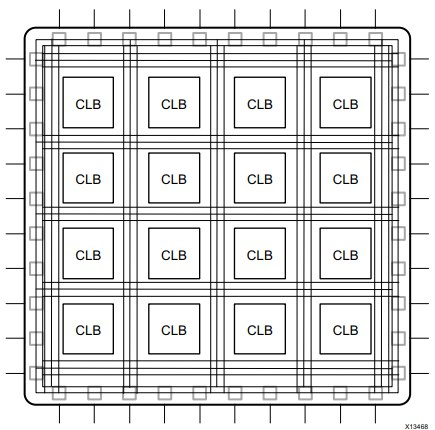
\includegraphics[width=12cm]{figuras/fpga-architecture.jpeg}
		}{
			\Fonte{\cite{fpgaxilinx}.}
		}	
	\end{figure}

Arquiteturas de FPGAs contemporâneas incluem blocos adicionais de \textit{interface}, armazenamento e de processamento específico, tais como blocos MAC, que aumentam a eficiência do dispositivo. Esses elementos adicionais são os seguintes:

\begin{itemize}
    \item Memórias Embarcadas para armazenamento distribuído de dados
    \item \textit{Phase-locked loops (PLLs)} para levar a \textit{FPGA Fabric} em diferentes taxas de clock
    \item Transceptores seriais de alta velocidade
    \item Controladores de memória \textit{Off-chip}
    \item Blocos multiplicadores-acumuladores (\textit{Multiply-accumulate blocks})
    
\end{itemize}

A combinação desses elementos fornece a FPGA a flexibilidade de implementar qualquer algoritmo de software em execução em um processador e representa a arquitetura de uma FPGA contemporânea.


\subsection{A FPGA Virtex Xilinx UltraScale+ VU9P} \label{sec:virtex}
 
 A Xilinx possui famílias de FPGAs, que são fabricadas em nós tecnológicos diversos, sendo as FPGAs \textit{high end} atualmente fabricadas no nó tecnológico de 16nm. A Tabela \ref{Tab:familias} mostra as famílias de acordo com os nós tecnológicos nos quais cada família é fabricada.

 Note que, conforme exemplificado acima com a Xilinx ultrascale+ fabricadas em 16nm, as FPGAs \textit{high end} são fabricadas em nós tecnológicos de dimensões menores, permitindo assim a integração de mais circuitos e unidades lógicas. De uma maneira geral, a FPGA  Virtex Xilinx UltraScale+ VU9P contém 1.182 LUTs, 2.364 flip-flops, 345.9 Mb de memória e 832 de I/O \cite{ultrascale}.

 A informação do custo de uma FPGA como esta não é fácil de se obter, é necessário entrar em contato com a \textit{Xilinx} e atender a pré-requisitos estabelecidos pela empresa para a informação ser oferecida. Porém, em discussões em fóruns e comunidades de desenvolvedores de aplicações para FPGA, estima-se que o custo é de entre $US$ 30,000 e $US$ 50,000. Contudo, é possível acessar aos recursos desta FPGA como um serviço, por meio da computação em nuvem, no ambiente de nuvem Amazon Web Services (AWS). Os conceitos de computação em nuvem e da AWS são discutidos a seguir.

 \begin{table}[!htb]
    \centering
    \caption{Famílias Xilinx de acordo com a tecnologia utilizada}
    \label{Tab:familias}
    \begin{tabular}{cccc}
    \hline 
    \textbf{45 nm}                        & \textbf{28 nm}   & \textbf{20 nm}    & \textbf{16 nm}                                                                                                                                                                                                                                            \\ \hline
    $Spartan & Virtex^{7} & Virtex Ultra Scale & Virtex Ultra Scale^{+}$
    
    \\ \hline
      & $Kintex^{7} & Kintex Ultra Scale & Kintex Ultra Scale^{+}$
     
     \\ \hline
     & $Artix^{7}$  &   &
     \\ \hline
     & $Spartan^{7}$  &   &
     \\ \hline
    \end{tabular}
   
\end{table}


\section{Computação em Nuvem}

Atualmente, os serviços básicos e essenciais como, água, eletricidade, telefone e gás, são entregues de uma forma transparente e são explorados por meio do modelo de pagamento baseado no uso. A mesma ideia tem sido utilizada com os serviços de informática. Neste sentido, plataformas e softwares estão sendo disponibilizados como serviços, por meio de um ambiente de Computação em Nuvem, melhorando a flexibilidade, reduzindo o custo do total do negócio e provendo serviços sob demanda.


A definição de Computação em Nuvem, ou \textit{Cloud Computing}, fornecida pelo National Institute of Standards and
Technology (NIST) diz que a Computação em Nuvem é um modelo para permitir acesso de rede conveniente e sob demanda a um conjunto compartilhado de recursos de computação configuráveis por exemplo, redes, servidores, aplicações de armazenamento  e serviços que podem ser rapidamente provisionados e liberados com esforço mínimo de gerenciamento ou interação com o provedor de serviços \cite{6203873}. Basicamente, a computação em nuvem move a computação e os dados para longe dos desktop e PCs portáteis convencionais para um grande \textit{data center}. Seu principal objetivo é fazer um melhor uso dos recursos distribuídos, combinando-os a fim de alcançar um maior rendimento, além de ser capaz de resolver a computação em grande escala.


A computação em nuvem apresenta cinco principais características, que são as seguintes:
\begin{itemize}
    \item \textit{Self-service} sob demanda: A capacidade dos consumidores em obter, configurar e implementar serviços na nuvem sem a necessidade de intervenção humana por parte do prestador de serviço.
    
    \item Amplo acesso: Diz respeito à disponibilidade dos recursos por meio de uma rede de computadores permitindo que diferentes dispositivos (computadores, tablets, smartphones, etc) possam acessae estes recursos através de mecanismos padronizados.   
    
    \item \textit{Pooling} de recursos: Os recursos de computação (armazenamento, processamento, memória, etc) do provedor de nuvem são agrupados para atender a diversos consumidores usando um modelo \textit{multi-tenant} (multi-inquilino), com diferentes recursos físicos e virtuais atribuídos e reatribuídos dinamicamente, de acordo com a demanda do consumidor.
    
    \item Elasticidade rápida: É a ideia dos recursos computacionais poderem ser rapidamente provisionados ou restringidos de acordo com a necessidade do consumidor.
    
    \item Serviço medido: A quantidade de recursos na nuvem usados pelo consumidor deve ser monitorada, controlada e reportada fornecendo transparência para o fornecedor e o consumidor do serviço utilizado.  Além disso, a partir dessa informação, devem ser estabelecidos os modelos de pagamento.

\end{itemize}


A crescente adoção da utilização de recursos provisionados pela nuvem por parte de pequenas e grandes empresas, se deve aos diversos benefícios que a computação em nuvem tem oferecido, como fácil gerenciamento, início rápido, escalabilidade, transparência de custos, baixo custo de manutenção, potencial para maior segurança, potencial para maior confiabilidade, etc. \cite{5942089}

Atualmente, empresas como a Amazon Web Services, Microsoft Azure, Google Cloud Platform e IBM Cloud fazem parte do grupo dos principais provedores de Computação em Nuvem. Na próxima seção serão discutidos os principais conceitos da Amazon Web Services, por se tratar do provedor que oferece o serviço estudado neste trabalho.  

\subsection{Amazon Web Services (AWS)}

A Amazon Web Services (AWS) é uma plataforma de computação formada por uma coleção de serviços de infra-estrutura, como poder de processamento, opções de armazenamento, redeQuando executa uma instância, o tipo de instância que você especifica determina o hardware do computador host usado para sua instância. Cada tipo de instância oferece uma memória de computação diferente e os recursos de armazenamento são agrupados em famílias de instâncias de acordo com esses recursos e banco de dados que são entregues como um utilitário: sob demanda, disponíveis em segundos, com preços pré-pagos \cite{awsOverview}.

Esses serviços operam a partir de 16 regiões geográficas pelo mundo, os mais centrais e conhecidos desses serviços são Amazon Simple Storage Service (S3), Amazon Elastic Compute Cloud (EC2) e Amazon Relational Database Service (RDS), estes dois primeiros foram utilizados neste estudo, e por isso, serão descritos a seguir.

\begin{itemize}

    \item \textbf{Amazon Simple Storage Service (S3)}: É um serviço de armazenamento de objetos criado para armazenar e recuperar qualquer quantidade de dados de qualquer local: sites e aplicativos móveis, aplicativos corporativos e dados de sensores ou dispositivos da IoT \cite{awsOverview}. Os objetos são organizados em \textit{buckets}, os são quais identificados por uma URI e acessados por meio de um serviço web.
    
    \item \textbf{Amazon Elastic Compute Cloud (EC2)}: Fornece acesso a instâncias (servidores) com recursos computacionais como um serviço sob demanda. O EC2 é uma parte essencial da AWS, pois fornece capacidade de computação escalável para as organizações. Estes são alguns dos recursos forneciso pelo EC2:
    \begin{itemize}
    \item Ambientes de computação virtual, conhecidos como instâncias.
    \item Os modelos pré-configurados para  instâncias, conhecidos como Imagens de máquina da Amazon (AMIs), que empacotam os bits necessários para o servidor (incluindo o sistema operacional e software adicional).
    \item Várias configurações de capacidade de CPU, memória, armazenamento e redes para as instâncias, conhecidas como tipos de instância.
    \item Informações seguras de login para as instâncias usando pares de chave (a AWS armazena a chave pública e o consumidor armazena a chave privada em um lugar seguro).
    \item Volumes de armazenamento para dados temporários que são excluídos quando uma instância é interrompida ou encerrada, conhecidos como volumes de armazenamento de instâncias.
    \item Volumes de armazenamento persistentes para os dados usando o Amazon Elastic Block Store (Amazon EBS), conhecidos como volumes do Amazon EBS.
\end{itemize}
 

Quando uma instância é executada, o tipo de instância especificada determina o hardware do computador host usado para a instância. Cada tipo de instância oferece uma memória de computação diferente e os recursos de armazenamento são agrupados em famílias de instâncias de acordo com esses recursos \cite{awsInstances}. O Amazon EC2 fornece os tipos de instâncias listados na Tabela \ref{Tab:Instancias}.

 
\begin{table}[H]
    \centering
    \caption{Tipos de instâncias do Amazon EC2}
    \label{Tab:Instancias}
    \begin{tabular}{ll}
    \hline 
    \textbf{Família de instâncias}                        & \textbf{Tipos de instância}                                                                                                                                                                                                                                                                                         \\ \hline
    \multicolumn{1}{|l|}{Propósito geral}                 & \multicolumn{1}{l|}{\begin{tabular}[c]{@{}l@{}}t2.nano | t2.micro | t2.small | t2.medium\\  | t2.large | t2.xlarge | t2.2xlarge | m4.large |\\  m4.xlarge | m4.2xlarge | m4.4xlarge | \\ m4.10xlarge | m4.16xlarge | m5.large |\\  m5.xlarge | m5.2xlarge | m5.4xlarge |\\  m5.12xlarge | m5.24xlarge\end{tabular}} \\ \hline
    \multicolumn{1}{|l|}{Otimizadas para computação}      & \multicolumn{1}{l|}{\begin{tabular}[c]{@{}l@{}}c4.large | c4.xlarge | c4.2xlarge | \\ c4.4xlarge | c4.8xlarge | c5.large | \\ c5.xlarge | c5.2xlarge | c5.4xlarge | \\ c5.9xlarge | c5.18xlarge\end{tabular}}                                                                                                       \\ \hline
    \multicolumn{1}{|l|}{Otimizado para memória}          & \multicolumn{1}{l|}{\begin{tabular}[c]{@{}l@{}}r4.large | r4.xlarge | r4.2xlarge | r4.4xlarge | \\ r4.8xlarge | r4.16xlarge | x1.16xlarge | \\ x1.32xlarge | x1e.xlarge | x1e.2xlarge | \\ x1e.4xlarge | x1e.8xlarge |x1e.16xlarge |\\  x1e.32xlarge\end{tabular}}                                                  \\ \hline
    \multicolumn{1}{|l|}{Otimizada para armazenamento}    & \multicolumn{1}{l|}{\begin{tabular}[c]{@{}l@{}}d2.xlarge | d2.2xlarge | d2.4xlarge | \\ d2.8xlarge | h1.2xlarge | h1.4xlarge | \\ h1.8xlarge | h1.16xlarge | i3.large | i3.xlarge | \\ i3.2xlarge | i3.4xlarge | i3.8xlarge | i3.16xlarge\end{tabular}}                                                             \\ \hline
    \multicolumn{1}{|l|}{Computação baseada em GPU, FPGA} & \multicolumn{1}{l|}{\begin{tabular}[c]{@{}l@{}}f1.2xlarge | f1.16xlarge | g3.4xlarge | \\ g3.8xlarge | g3.16xlarge | p2.xlarge | \\ p2.8xlarge | p2.16xlarge | p3.2xlarge | \\ p3.8xlarge | p3.16xlarge\end{tabular}}                                                                                               \\ \hline
    \end{tabular}
   
\end{table}



\end{itemize}

\section{O Serviço Amazon EC2 F1  de Processamento remoto  em   FPGAs na nuvem}\label{sec:servicos amazon}

    Com a grande quantidade de tecnologias e plataformas que estão sendo apresentadas no mercado, os centros de dados dessas aplicações cada vez mais precisam enfrentar o desafio de acelerar cargas de trabalho com tipos de dados complexos, que exigem um poder de processamento que ultrapassa a capacidade de CPUs tradicionais.
    
    As GPUs são amplamente usadas para o processamento de aplicações de análise de dados e de aprendizagem de máquinas. As FPGAs tem sido vistas como uma melhor solução, proporcionando maior desempenho por watt em vários cenários \cite{8119247}, em particular naqueles que fazem uso de aritmética de ponto fixo e não realizam operações de ponto flutuantes. No entanto, a adoção de FPGAs para aceleração de aplicações ainda é limitada devido a dificuldade de implementação tanto de um acelerador eficiente baseado em FPGA,  quanto da infra-estrutura que realiza a comunicação entre o acelerador e a aplicação que fornece e/ou recebe dados da FPGA. 
    
    A fim de facilitar essa comunicação e oferecer um ambiente pronto para o desenvolvimento de acelerações baseadas em FPGAs, a AWS lançou no ano de 2016 as instâncias de computação em nuvem Elastic Compute Cloud (EC2) F1, que são equipadas com FPGAs Xilinx. Essas instâncias permitem uma maior rapidez no desenvolvimento das aplicações por disponibilizarem todos os itens necessários para desenvolver, simular, depurar e compilar código de aceleração de hardware \cite{aws2016f1}.
    
    
    
    Abaixo serão descritos todos os conceitos necessários para o desenvolvimento e implementação de acelerações baseadas em FPGAs, fornecidas pelo AWS EC2 F1.
    
    

  
\subsection{Arquitetura da instância F1} \label{sec:arq}
    
    A implantação do design da aplicação para a FPGA é feita nas instâncias EC2 F1, que são oferecidas em dois tamanhos diferentes e disponibilizam FPGAs Xilinx UltraScale+ VU9P fabricadas em tecnologia de 16 nm. É possível iniciar múltiplas instâncias com 1 ou 8 FPGAs conectadas. Cada placa inclui 64 GiB de memória protegida DDR4 ECC com uma conexão PCIe x16 dedicada.  Cada FPGA contém aproximadamente 2,5 milhões de elementos de lógica e 6.800 mecanismos de processamento de sinais digitais (DSP) \cite{aws2016f1}. % verificar essa citação do site
    
    As especificações mais detalhadas de cada tipo de instâncias F1 são mostradas na Tabela \ref{Tab:F1}. 
        
    \begin{table}[!htb]\tiny
    \centering
     \caption{Detalhes da Instância F1}
    \label{Tab:F1}
    \begin{tabular}{lccccccc}
    \hline
    \multicolumn{1}{l}{Tipo de Instância}&\multicolumn{1}{l}{FPGAs }&\multicolumn{1}{l}{DDR-4(Gib)}&\multicolumn{1}{l}{vCPUs}&\multicolumn{1}{l}{Memória (GiB)}&\multicolumn{1}{l}{Arm. NVMe (GB)}&\multicolumn{1}{l}{Largura de Banda} \\ \midrule 
    
    f1.2xlarge & 1 & 4 x 16 & 8 & 122 & 1 x 470 & Até 10 Gbps\\   \midrule
    f1.16xlarge & 8 & 32 x 16 & 64 & 976 & 4 x 940 & 25  Gbps\\   \midrule

    \end{tabular}
    \end{table}
    


A aceleração baseada em FPGA na AWS é uma estratégia de coprocessamento, a FPGA é ligada aos pós-processadores via PCI Express (PCIe), essa conexão PCIe também permite a comunicação entre as FPGAs da instância f1.16xlarge. Assim, uma típica aplicação para a instância f1 inclui um software executando nos processadores host comunicando dados e instruções, através de uma interface PCIe, para a FPGA, que contém a aplicação que foi desenvolvida e carregada na FPGA. A Figura \ref{fig:f1-architecture} detalha esse processo de comunicação.


   
\begin{figure}[h!] 
   	    \captionsetup{width=12cm}%Da mesma largura que a figura
		\Caption{\label{fig:f1-architecture} Como uma aceleração de FPGA funciona na AWS}
		\UFCfig{}{
			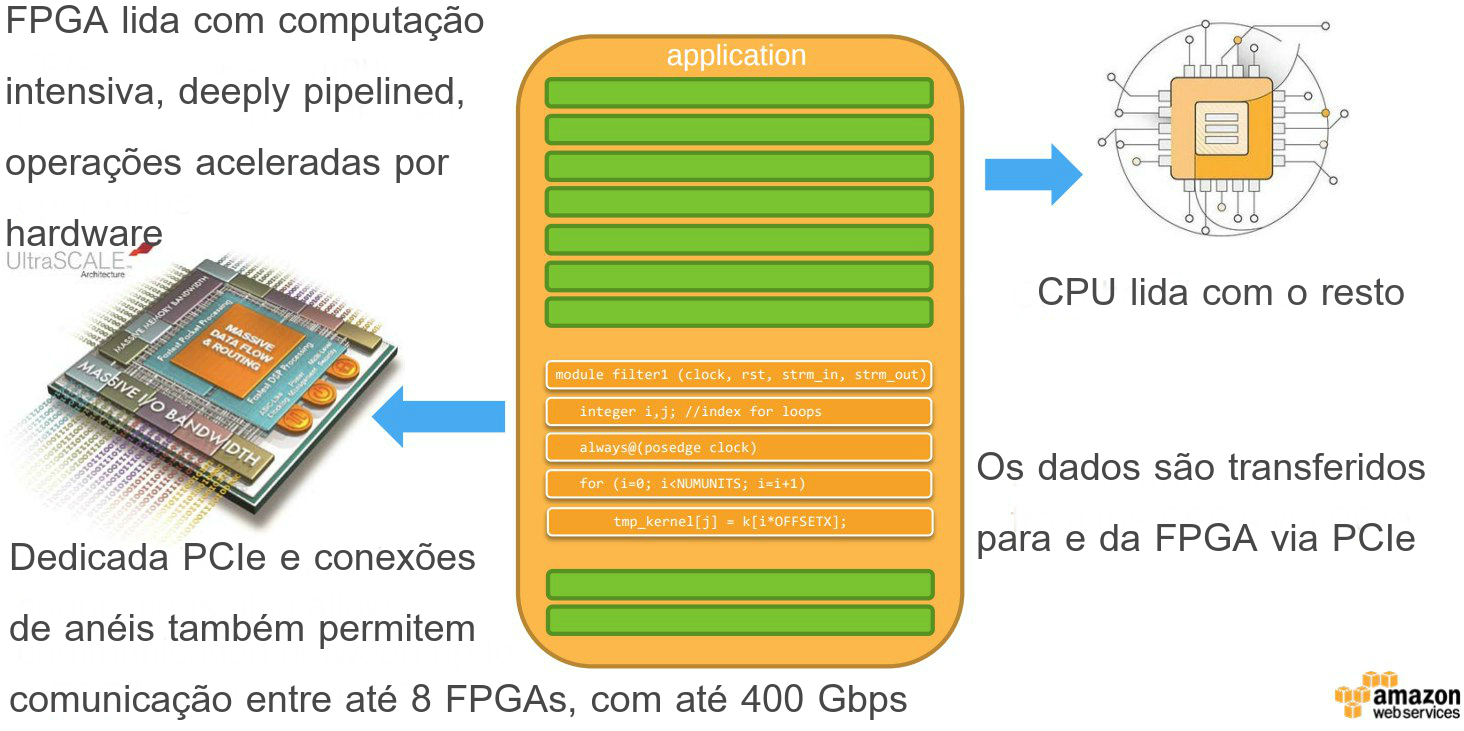
\includegraphics[width=12cm]{figuras/f1-architecture.jpg}
		}{
			\Fonte{\cite{aws2016f1}.}
		}	
	\end{figure}
    

\subsection{Desenvolvimento de Cores} \label{sec:dev}

Para desenvolver as aplicações FPGAs é necessário seguir um fluxo de programação proposto pela AWS. Esse fluxo é descrito pelos seguintes passos:

\begin{enumerate}
    \item Desenvolver a \textbf{Lógica Customizada (\textit{Custom Logic - CL)}} para a FPGA utilizando as ferramentas de desenvolvimento da Xilinx, disponíveis na \textbf{\textit{FPGA Deveploper AMI}}, combinadas com o \textbf{Kit de desenvolvimento - HDK }.
    
    \item Combinar a CL com uma lógica fornecida pela AWS chamada de \textbf{FPGA \textit{Shell}}.
    
    \item Criar uma \textbf{\textit{Amazon FPGA Image (AFI)}} a partir da CL construída.
    
    \item Carregar a AFI gerada em uma FPGA conectada à instância F1 ou disponilizar no AWS Marketplace.
\end{enumerate}

Os recursos ofertados pela AWS citados na descrição do fluxo de desenvolvimento serão discutidos nas próximas seções.

\subsubsection{ FPGA Developer AMI} \label{sec:ami}

Para permitir um desenvolvimento rápido de acelerações de hardware, a AWS disponibiliza uma AMI para desenvolvedores de FPGA, a \textit{FPGA Developer AMI}, que é um ambiente de desenvolvimento pré-definido, com scripts e ferramentas para o desenvolvimento, compilação e simulação do design FPGA, pronto para ser executado em uma instância EC2. Por se tratar de uma ambiente de desenvolvimento, \textit{FPGA Developer AMI} normalmente não é executada em uma instância F1, mas em outros tipos de instâncias EC2, em uma instância que não contém uma FPGA. A AMI pode ser implantada em uma variedade de tipos e tamanhos de instâncias EC2, como por exemplo a M4 que é para propósitos gerais, a R4 que é otimizada para memória, a C4 que é otimizada para computação, ou a T2, que tem um baixo custo. esta última deve ser usada apenas para o design e simulação, não sendo indicada para a síntese ou PAR (\textit{place-and-route}).

\textit{FPGA Developer AMI} está disponível no AWS Marketplace, onde não são aplicados custos para o uso da AMI e suas ferramentas, apenas são cobrados os custos por hora de execução da instância EC2 escolhida.


\subsubsection{Kit de desenvolvimento - HDK e SDK} \label{sec:hdk}
    
    A AWS disponibiliza o repositório AWS-FPGA na plataforma github, no endereço https://github.com/aws/aws-fpga, que contém os kits de desenvolvimento de hardware e software. Esses kits incluem duas partes: o HDK e o SDK.
    
    O HDK é um diretório onde estão disponíveis todos os arquivos de design e scripts necessários para criar uma \textit{Amazon FPGA Image (AFI)} a partir de um projeto RTL(Verilog/VHDL), que é uma imagem que contém o bitstream pronto para ser implementado em uma FPGA. Para usá-lo, o desenvolvedor deve baixar o HDK instalá-lo em seu ambiente de desenvolvimento, na nuvem ou local.
    
    Nesse diretório estão inclusos todos os scripts de criação do ambiente de desenvolvimento, simulação, compilação e criação da AFI. A instalação do HDK pode ser feita em qualquer servidor local ou em uma instância EC2. O uso do HDK é necessário apenas se for preciso criar uma AFI e não utilizar uma AFI pré-construída.
    
    O diretório SDK inclui todos os drives e o ambiente de execução exigidos em qualquer instância EC2 FPGA. Esses drives e ferramentas são usados para a interação com as AFI pré-construídas que serão carregadas nas FPGAs disponíveis nas instâncias EC2 F1.
    
    Além disso, o SDK contém as ferramentas de gerenciamento da \textit{Amazon FPGA Image (AFI)}, que inclui tanto o código fonte para as ferramentas de gerenciamento da AFI, quanto as descrições detalhadas dos comandos a serem usados  uma instância F1.
    

     
\subsubsection{Lógica Customizada (Custom Logic - CL)} \label{sec:cl}

A Lógica Customizada, ou \textit{Custom Logic - CL}, é o design completo desenvolvido para a FPGA. A combinação da CL com a AWS Shell tem como resultado um \textit{Design Checkpoint (DCP)} e não um bitstream, esse é gerado pela AWS depois que o desenvolvedor envia o DCP \cite{awsfaq}. 

Existe uma interface entre a CL e uma aplicação real em execução no espaço do usuário do linux durante o tempo de execução. Nessa interface há duas partes: \textit{Management} e \textit{Runtime}. A Figura \ref{fig:cl} mostra uma visão de alto nível desses componentes e como eles se relacionam com a FPGA.

\begin{figure}[htb!] 
   	    \captionsetup{width=15cm}%Da mesma largura que a figura
		\Caption{\label{fig:cl} Visão do programador da Custom Logic}
		\UFCfig{}{
			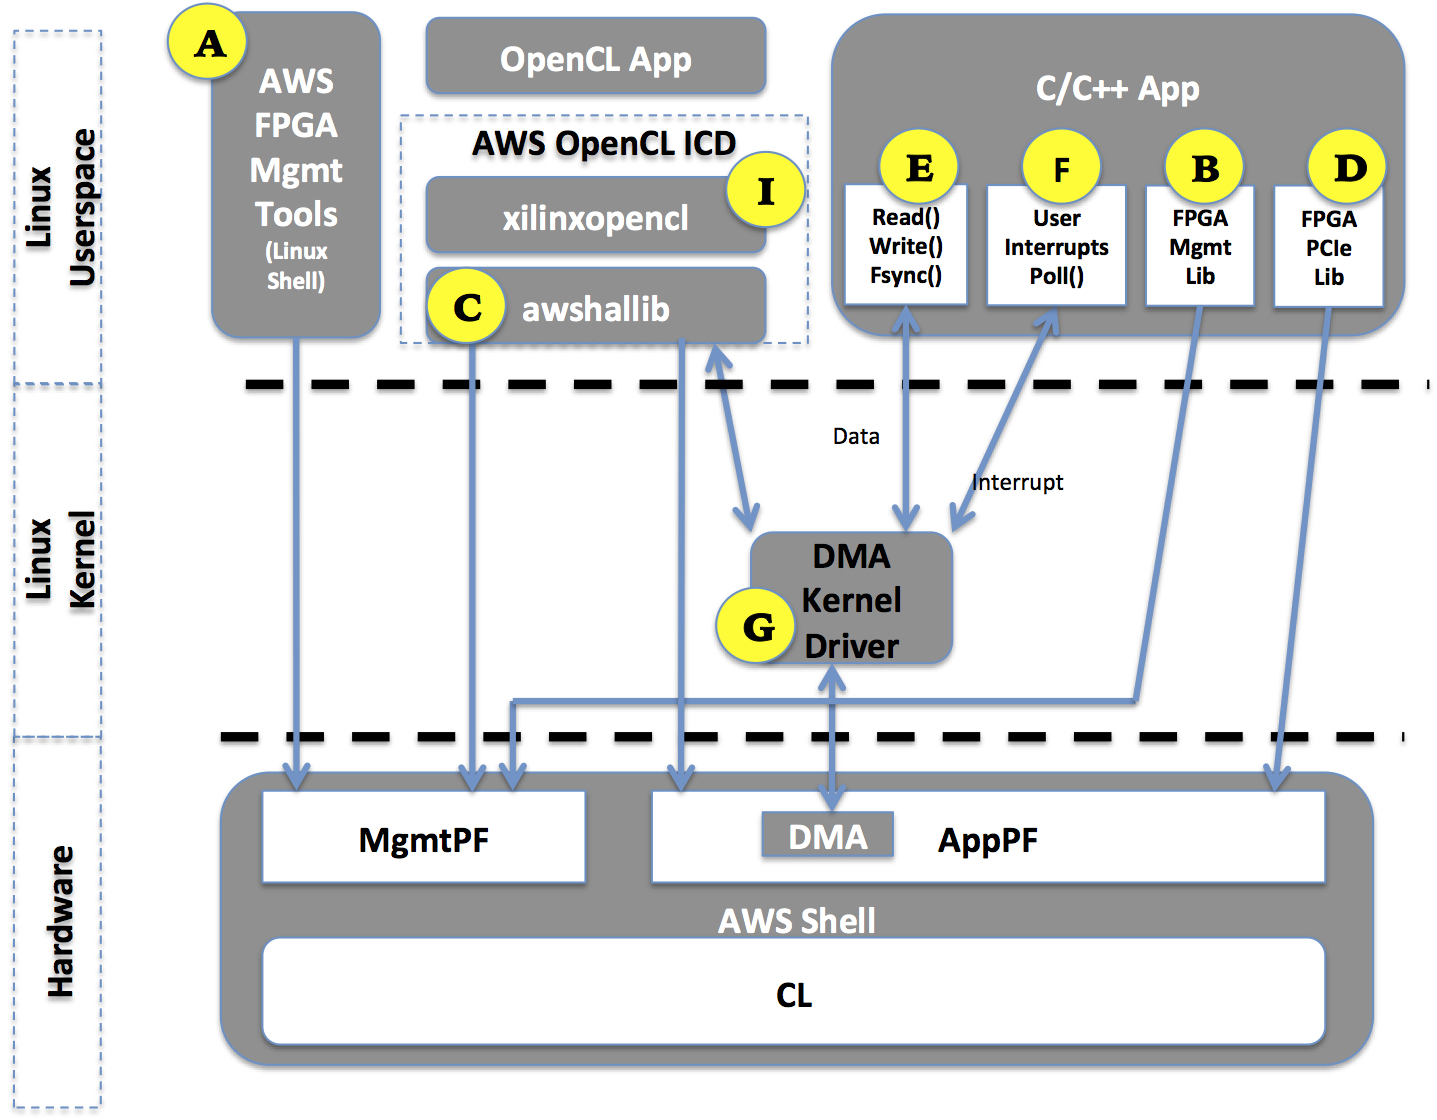
\includegraphics[width=16cm]{figuras/cl.png}
		}{
			\Fonte{\cite{awscl}.}
	}		
\end{figure}

\begin{enumerate}
    \item \textbf{Management Interface}: necessário para carregar/limpar uma AFI, verificar o status de uma AFI, depurar a AFI, os LEDs Emulados e os  DIP Switches Emulados \cite{awscl}. A interface de gerenciamento é fornecida em uma das três opções, uma ou mais podem ser usadas simultaneamente:
    
   \textbf{[A]} Como comandos shell do linux chamados de  FPGA Management Tools. 
    
    \textbf{[B]} Como uma biblioteca C chamada de FPGA Management Lib para ser compilada com a aplicação C/C++ do desenvolvedor.
    
    \textbf{[C]} Pré-integrado com OpenCL runtime library.
    
    \item \textbf{Runtime Code}: necessário para leitura/gravação de/para a lógica personalizada, tratamento de interrupções e uso do DMA \cite{awscl}. Isso é fornecido por:
    
    \textbf{[D]} FPGA PCIe Lib é uma biblioteca C usada para acessar o espaço de memória da FPGA atrás do AppPF PCIe BARs (definidos no FPGA Shell), do espaço de aplicação Linux, como leitura/gravação, para registrar espaço ou transmitir mensagens. Esta biblioteca pode ser compilada e vinculada na aplicação C/C++ do desenvolvedor.
    
    \textbf{[E]} Uma  Interface DMA usando padrão  POSIX API como open()/read()/write() para ser usada em qualquer aplicação C/C++ para transferência de dados usando DMA. Essa interface de DMA requer a instalação do driver de kernel  AWS EDMA - marcado como item \textbf{[G]}.
    
    \textbf{[F]} Um Espaço de usuário de notificação interrupção/evento usando padrão  POSIX API like open() and poll(), para ser usado em qualquer aplicação C/C++. Essa interface interrupção/evento requer a instalação do driver de kernel  AWS EDMA - marcado como item \textbf{[G]}.
    
    \textbf{[I]} Uma biblioteca OpenCL ICD que se vincula a aplicação de tempo de execução openCL, como o gerado pelo SDAccel da Xilinx.
    

\end{enumerate}



\subsubsection{FPGA Shell} \label{sec:shell}

O \textit{AWS Shell} é a parte da FPGA que é fornecida e gerenciada pela AWS. É uma Lógica responsável por cuidar dos periféricos externos FPGA, PCIe, DRAM e Interrupções.Ele  implementa as tarefas não diferenciadas de desenvolvimento e de trabalho pesado, como configurar a interface PCIe, download de AWS FPGA Image, segurança, monitoramento de integridade, métricas e ganchos de depuração \cite{awsfaq}. Cada FPGA implantada na nuvem inclui um AWS Shell e as interfaces da \textit{custom logic} do desenvolvedor com as interfaces disponíveis do AWS Shell.

A Tabela \ref{Tab:shell} e a Figura \ref{fig:shell}  resumem as várias interfaces entre o Shell e o CL.



\begin{figure}[H] 
   	    \captionsetup{width=15cm}%Da mesma largura que a figura
		\Caption{\label{fig:shell} Interfaces Shell}
		\UFCfig{}{
			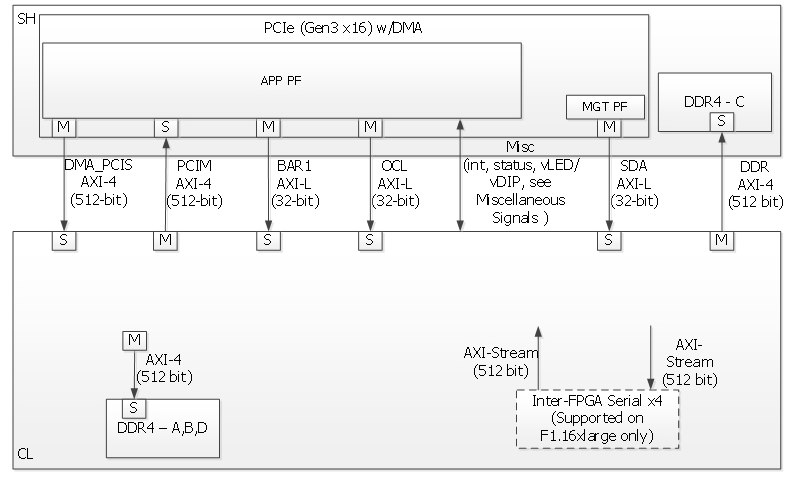
\includegraphics[width=16cm]{figuras/shell.jpeg}
		}{
			\Fonte{\cite{awsshell}.}
	}		
\end{figure}


      
\begin{table}[H]
    \centering
     \caption{Interfaces Shell}
    \label{Tab:shell}
     \begin{tabular}{|l|l|}
    \hline
    \textbf{Interface} & \textbf{Descrição}                                                                                                                    \\ \hline
    Clocks e Resets    & Existem vários clocks e resets fornecidos pelo Shell para o CL                                                                        \\ \hline
    DDR4               & \begin{tabular}[c]{@{}l@{}}A interface principal para os controladores DDR4 utiliza uma\\  interface AXI-4\end{tabular}               \\ \hline
    DMA\_PCIS          & \begin{tabular}[c]{@{}l@{}}A interface PCIe Slave (PCIS) é uma interface AXI-4 usada \\ para transações PCIe de entrada\end{tabular}  \\ \hline
    PCIM               & \begin{tabular}[c]{@{}l@{}}A interface PCIe Master (PCIM) é uma interface AXI-4 usada \\ para transações PCIe de saída\end{tabular}   \\ \hline
    SDA                & \begin{tabular}[c]{@{}l@{}}A interface SDA é uma interface AXI-Lite associada ao MgmtPF\\  e ao BAR4\end{tabular}                     \\ \hline
    OCL                & \begin{tabular}[c]{@{}l@{}}A interface OCL é uma interface AXI-Lite associada ao AppPF e \\ ao BAR0\end{tabular}                      \\ \hline
    BAR1               & \begin{tabular}[c]{@{}l@{}}The BAR1 Interface is an AXI-Lite interface associated with AppPF\\  and BAR1\end{tabular}                 \\ \hline
    Interrupts         & Existem 16 interrupções de usuário disponíveis                                                                                        \\ \hline
    Miscellaneous      & \begin{tabular}[c]{@{}l@{}}Existem vários sinais genéricos, como ID's, status, contadores, etc.,\\ entre o Shell  e o CL\end{tabular} \\ \hline
    \end{tabular}
\end{table}

A plataforma FPGA da F1 inclui as seguintes interfaces externas:

\begin{itemize}
    \item Um x16 PCI Express 3.0 Interface.
    \item 
Quatro interfaces DDR4 RDIMM, cada interface é de 72 bits, incluindo ECC.
\end{itemize}
 
Em relação a representação PCIe FPGA para instância do EC2, Existem duas funções físicas PCIe (Physical Functions - PFs) apresentadas à instância F1:

\begin{itemize}
    \item Management PF - Essa PF é usada para o gerenciamento da FPGA e as bibliotecas de gerenciamento FPGA. a Management PF fornece acesso a várias funções de controle, como Virtual-LED, Virtual-DIPSwitch, JTAG virtual, métricas de FPGA e gerenciamento de AFI (carga, limpeza, etc ...) \cite{awsshell}.
    
    \item Application PF (AppPF) - A AppPF é usado para funcionalidades específica do CL.
\end{itemize}

\paragraph{Amazon FPGA Image (AFI)} \label{sec:afi}
 
 Uma \textit{Amazon FPGA Image} é o código FPGA compilado que é carregado em um FPGA na AWS para executar a CL criada pelo desenvolvedor. As AFIs são mantidas pela AWS de acordo e associados à conta da AWS que os criou. O AFI inclui o CL e o \textit{AWS FPGA Shell} \cite{awsfaq}.
 
 Após a conclusão do design, é possível registrar uma Amazon FPGA Image (AFI), que é uma imagem de FPGA que será carregada na FPGA conectada à instância e poderá ser reusada muitas vezes e em quantas instâncias F1 for desejadas.  

Após o processo da criação de uma AFI são fornecidos as seguintes identificadores referentes a AFI criada :
\begin{itemize}

\item FPGA Image Identifier ou AFI ID: este é o ID principal, usado para gerenciar a AFI através dos comandos AWS EC2 CLI e AWS SDK APIs. Este ID é regional, ou seja, se uma AFI é copiado em várias regiões, ele terá uma  AFI ID única diferente em cada região. Um exemplo de AFI ID é afi-06d0ffc989feeea2a. 

\item Global FPGA Image Identifier ou AGFI ID: esta é uma identificação global que é usada para se referir a uma AFI dentro de uma instância F1. Por exemplo, para carregar ou limpar um AFI de um slot FPGA, você usa o AGFI ID. Uma vez que as  AGFI  IDs são globais (por design), permite copiar uma combinação de AFI / AMI para várias regiões, e elas funcionarão sem requerer nenhuma configuração adicional. Um exemplo AGFI ID é agfi-0f0e045f919413242.

\end{itemize}


\subsection{Tarifação} \label{sec:tarifacao}

Os custos gerados ao desenvolver um aplicação para FPGA na AWS dizem respeito a quantidade de horas que as instâncias, usadas para o desenvolvimento e a instância F1, são executadas. Cada instância tem um custo por hora. As instâncias F1 apresentam os seguintes custos:

\begin{itemize}
    \item f1.2xlarge: USD\$1.65 por hora.
    
    \item f1.16xlarge: USD\$13.2 por hora.
\end{itemize}


    




	\chapter{Metodologia de Desenvolvimento}
\label{chap:metodologia}

Neste capítulo detalha-se o trabalho proposto por essa monografia, um estudo sobre a utilização das instâncias EC2 F1 como recurso didático para a disciplina de Sistemas Eletrônicos Digitais Reconfiguráveis (SEDR) do curso de Engenharia de Computação da Universidade Federal do Ceará. Serão apresentadas a metodologia utilizada, todas as práticas realizadas e as ferramentas utilizadas.

\section{Metodologia Utilizada}\label{sec: metodologia-utilizada}

A metodologia adotada para a execução deste trabalho é mostrada nas etapas mostradas da Figura \ref{fig:metodologia}:



\begin{figure}[htb!] 
   	    \captionsetup{width=15cm}%Da mesma largura que a figura
		\Caption{\label{fig:metodologia}{Metodologia}}
		\UFCfig{}{
			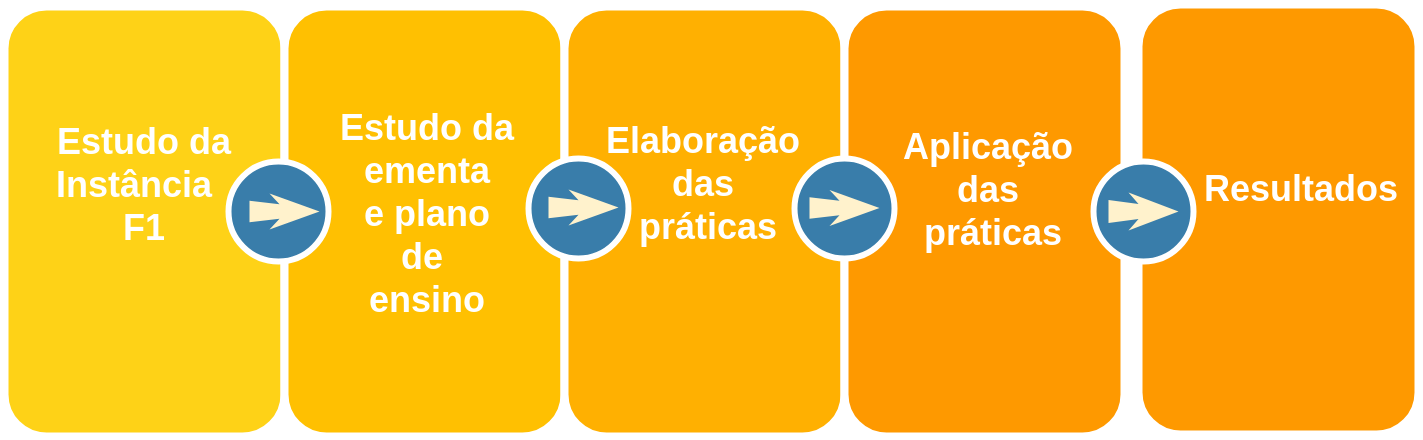
\includegraphics[width=16cm]{figuras/metodologia.png}
		}{
			\Fonte{Próprio Autor.}
	}		
\end{figure}
    
\begin{enumerate}
    \item \textbf{Estudo da Instância F1:} Primeiramente, foi realizado um estudo das instâncias EC2 F1 com o intuito de identificar as possibilidades que esse recurso poderia oferecer para o seu uso no ensino de FPGA.
    
    \item \textbf{Estudo da ementa e plano de ensino da Disciplina de SEDR:} Em seguida, deu-se início ao estudo da ementa e do plano de ensino da disciplina de SEDR para que a utilização das instâncias EC2 F1 fosse adequada da melhor forma possível ao plano de ensino.
    
    \item \textbf{Elaboração das práticas:} Baseando-se nos estudos já realizados e na documentação da Amazon Web Services, as práticas de laboratório foram idealizadas de forma a oferecer um conhecimento geral do processo de desenvolvimento de aplicações para FPGA com o serviço EC2 F1.
    
     \item \textbf{Criação da máquina virtual:} Com a finalidade de abordar o desenvolvimento local (\textit{on-premises}) com o kit de desenvolvimento da AWS \cite{on-premises} nas práticas 3 e 4, uma máquina virtual foi criada e configurada para conter o kit de desenvolvimento da AWS, o HDK e o SDK, e o ambiente de desenvolvimento da Xilinx SDSoC 2017.1 op, que contém o Vivado com uma licença específica para a FPGA Virtex UltraScale+ VU9P.
    
    \item \textbf{Aplicação das práticas:} Após a elaboração e testes das práticas, iniciou-se a fase de aplicação em laboratório.
    
    \item \textbf{Resultados:} Finalmente, nesta última etapa da metodologia foi analisada a eficácia do uso das instâncias EC2 F1, como recurso didático para a disciplina de SEDR, através da aplicação das práticas, e de análise de questionários respondidos pelos alunos ao final de cada prática.
	  
\end{enumerate}

  
\section{Contextualização}\label{sec: contextualizacao}

O trabalho foi realizado no Departamento de Teleinformática da Universidade Federal do Ceará. As práticas foram aplicadas em dois laboratórios deste mesmo departamento para alunos de graduação.

As práticas foram aplicadas na disciplina de SEDR, que é um componente optativo da estrutura curricular do Curso de Graduação em Engenharia de Computação e é ofertada no sétimo semestre da graduação, tendo a carga horária de 64 horas (vide ANEXO \ref{an:ex_anexo_a}) e tinha o total de 11 alunos matriculados. Dos quais, 2 alunos realizaram o trancamento da disciplina, 1 é a autora deste trabalho e, portanto, 8 alunos realmente realizaram as práticas. 

De acordo com a ementa, a carga horária total da disciplina é dividida igualmente entre teoria e prática, ou seja, são utilizadas 32 horas para a teoria e 32 horas para a pŕatica. A carga horária reservada para a  aplicação das práticas desenvolvidas neste trabalho foi de 10 horas, dessa quantidade, 2 horas foram utilizadas para uma aula teórica sobre a Amazon Web Services (AWS) e o serviço EC2 F1 e as 8 horas restantes foram reservadas para a aplicação das práticas, levando em consideração apenas as atividades desenvolvidas no laboratório durante o horário da aula.

As práticas foram realizadas no Laboratório de Informática e no Laboratório de Hardware do Departamento de Teleinformática. No primeiro, foram realizadas as práticas 1 e 2 que usam o acesso remoto às instâncias F1. As práticas 3 e 4 foram realizadas no Laboratório de Hardware, onde foram instaladas imagem das máquinas virtuais que permitem  o desenvolvimento local (\textit{on premises}) das práticas.

\section{Ferramentas Utilizadas}\label{sec: ferramentas}

Esta Seção detalha as ferramentas que foram utilizadas para a realização das atividades de labotório.

\subsection{Software}\label{sec: software}

\subsubsection{AWS Command Line Interface (CLI)}\label{sec: aws-cli}

A AWS \textit{Command Line Interface} (CLI) é uma ferramenta de código aberto que fornece comandos para interagir com os serviços da Amazon Web Services \cite{awscli}. Após a sua configuração, é possível gerenciar todos os recursos fornecidos pela AWS, pois é fornecido o acesso direto a APIs públicas de serviços da AWS. Esse acesso pode ser realizado por meio de comandos ou scripts de shell, ou até mesmo com programas em várias linguagens de programação, utilizando o SDK da AWS. Neste projeto, utilizou-se a AWS CLI para a iniciar instâncias pelo terminal, criar \textit{buckets} no S3 e armazenar o DCP gerado nesses \textit{buckets}.   

\subsubsection{GitHub}\label{sec: github}
o GitHub é uma plataforma de hospedagem de código-fonte que  utiliza o sistema de controle de versão distribuído Git. Ele é usado para armazenar o código-fonte de um projeto e rastrear o histórico completo de todas as alterações feitas nesse código. Além disso, é amplamente utilizado para divulgação e/ou contribuição de trabalhos. O GitHub foi utilizado neste trabalho para armazenar as alterações feitas pelos alunos no repositório da AWS, para que posteriormente o projeto modificado pudesse ser copiado para a máquina em que a prática estava sendo desenvolvida.

\subsubsection{Vivado Design Suite}\label{sec: vivado}
O Vivado Design Suite é um pacote de software produzido pela Xilinx que permite a edição, síntese, análise e simulação de um projeto para FPGA. Ele foi usado neste trabalho para o desenvolvimento dos projetos de FPGAs abordados nas práticas.

\subsubsection{VMware}\label{sec: vmware}

VMware um software/máquina virtual que permite a instalação e utilização de um sistema operacional dentro de outro \cite{vmware}. A fim de abordar o desenvolvimento \textit{on premises} usando os recursos da AWS, criou-se uma máquina virtual que continha todas as ferramentas, com suas devidas licenças, todas gratuitas,instaladas. O VMware foi utilizado para executar essa máquina virtual criada.

\subsection{Hardware}\label{sec: Hardware}

Utilizou-se os computadores do Laboratório de Informática, com sistemas operacional Linux, e o os computadores do Laboratório de Hardware com o sistema operacional Windows instalado.


\section{Estrutura das aulas de laboratório}
Como apresentado na Seção \ref{sec: contextualizacao}, as práticas 1 e 2 foram realizadas no Laboratório de Informática, utilizando as máquinas do próprio laboratório para fazer o acesso remoto às instâncias da AWS. Durante essas práticas os alunos acessam, via SSH da máquina local, a instância t2.2xlarge para desenvolverem seu projeto, gerar o DCP e criar a AFI, a ser gravada na FPGA. Após isso, a instância f1.2xlarge, a qual contém a placa com a FPGA, é acessada via ssh e finalmente, a AFI é gravada na FPGA conectada à instância. A Figura \ref{fig:praticas-1e2} mostra o procedimento descrito.

Para a realização das práticas 3 e 4 utilizou-se uma máquina virtual para realizar o desenvolvimento local. Nessa máquina, foram executados os comandos necessários para a criação e simulação do projeto, no caso da prática 3. Na prática 4 os comandos executados realizaram a simulação, a síntese e a conexão com a interface Shell. As Figuras \ref{fig:pratica3} e \ref{fig:pratica4} mostram a estrutura das práticas 3 e 4, respectivamente.

\begin{comment}
\begin{figure}[htb!] 
   	    \captionsetup{width=6cm}%Da mesma largura que a figura
		\Caption{\label{fig:praticas-1e2} Estrutura das práticas 1 e 2.}
		\UFCfig{}{
			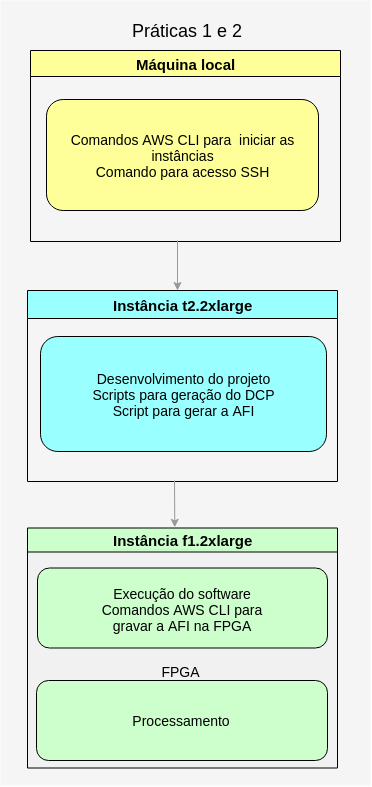
\includegraphics[width=7cm]{figuras/Praticas1e2.png}
		}{
			\Fonte{Próprio Autor.}
	}		
\end{figure}

\begin{figure}[htb!] 
   	    \captionsetup{width=7cm}%Da mesma largura que a figura
		\Caption{\label{fig:pratica3} Estrutura da prática 3.}
		\UFCfig{}{
			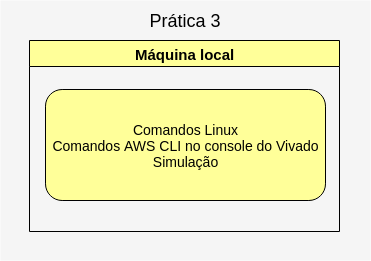
\includegraphics[width=8cm]{figuras/pratica3.png}
		}{
			\Fonte{Próprio Autor.}
	}		
\end{figure}

\begin{figure}[htb!] 
   	    \captionsetup{width=7cm}%Da mesma largura que a figura
		\Caption{\label{fig:pratica4} Estrutura da prática 4.}
		\UFCfig{}{
			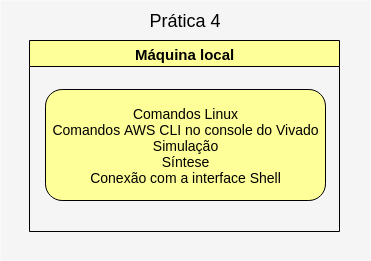
\includegraphics[width=8cm]{figuras/pratica4.png}
		}{
			\Fonte{Próprio Autor.}
	}		
\end{figure}
\end{comment}

\begin{figure}[h!]
\begin{minipage}{0.48\columnwidth}
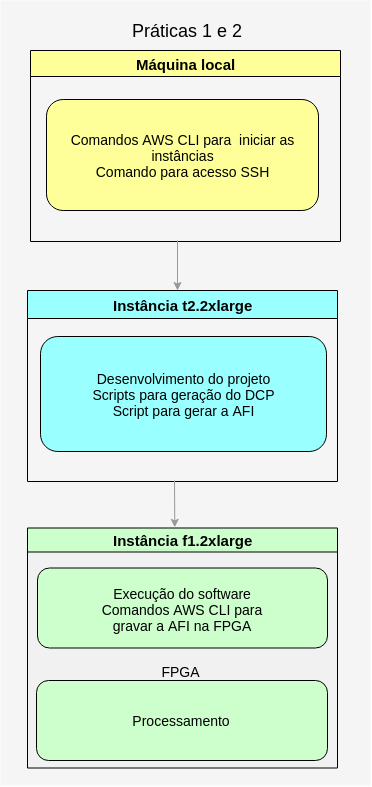
\includegraphics[width=\columnwidth,height=150mm]{figuras/Praticas1e2.png}
\end{minipage}
\begin{minipage}{0.48\columnwidth}
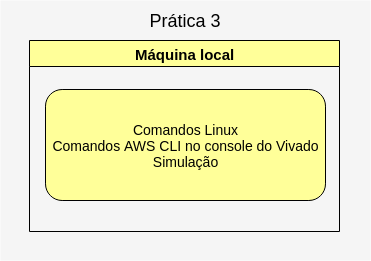
\includegraphics[width=\columnwidth,height=6cm]{figuras/pratica3.png}
\\[5mm]
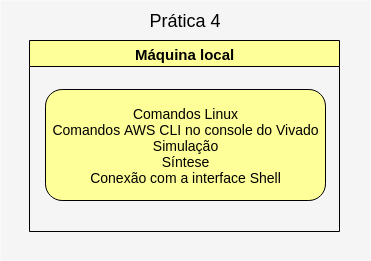
\includegraphics[width=\columnwidth,height=6cm]{figuras/pratica4.png}
\end{minipage}
\Fonte{Próprio Autor.}
\end{figure}



\section{Proposta de Práticas de Laboratório Para a Discplina de SEDR}

Após a realização de uma etapa de estudos sobre a utilização do serviço EC2 F1 da AWS, deu-se início ao estudo da ementa (vide ANEXO \ref{an:ex_anexo_a}) e do plano de ensino  da disciplina de SEDR, como citado na Seção \ref{sec: metodologia-utilizada}. Com base nesses estudos, foram propostas algumas práticas de laboratório que fossem factíveis, considerando-se limitações de tempo e de recursos financeiros para o acesso às instâncias da AWS, e que pudessem abordar o procedimento para o desenvolvimento de projetos em FPGA, na nuvem, de maneira satisfatória. Como resultado, chegou-se a um conjunto de quatro práticas que serão descritas a seguir. Maiores detalhes das práticas podem ser vistos nos roteiros de cada uma, disponíveis no Anexo deste documento e na plataforma GitHub, no link: \url{https://github.com/vanros/Praticas-SEDR-AWS}.

\subsection{Prática 1: Criação de uma Amazon FPGA Image (AFI) do exemplo CL hello world}

\noindent\textbf{\textit{Objetivo}}

O objetivo dessa prática foi apresentar o uso do serviço EC2 F1 da AWS, abordando a conexão e configuração das instâncias t2.2xlarge e f1.2xlarge, além de todos os procedimentos necessários para a execução de um projeto exemplo utilizando a FPGA conectada à instância f1.2xlarge.


\noindent\textbf{\textit{Breve descrição}}

Nesta prática foi utilizado um exemplo do repositório da AWS para realizar o procedimento de geração do DCP,  geração da AFI e a execução do software que se comunica com a FPGA. Nesse exemplo, o valor 0xEFBEADDE é escrito em um registrador, após isso a FPGA ler o mesmo registrador, realiza um \textit{byte swap}, alterando o valor para 0xDEADBEEF, que será lido posteriormente pelo software. Também são demonstrados os recursos de Virtual LED e DIP switch, oferecidos pelo Shell.

\subsection{Prática 2: Implementando um somador a partir do exemplo CL hello world}

\noindent\textbf{\textit{Objetivo}}

O objetivo dessa prática foi abordar a implementação de um somador a partir do código do exemplo CL hello world e executar esse somador na FPGA conectada à instância f1.2xlarge.

\noindent\textbf{\textit{Breve descrição}}

Nesta prática foi implementado uma soma de dois valores, a partir do exemplo CL 
Hello world. Foram declarados dois endereços de registradores, na interface BAR0/OCL, para os quais devem ser enviados os valores a serem somados, e um registrador para armazenar o resultado da soma.

\subsection{Prática 3: Executando e simulando o exemplo CL hello world com a GUI do Vivado}

\noindent\textbf{\textit{Objetivo}}

O objetivo foi acessar a interface gráfica do vivado instalado na instância t2.2xlarge e utilizá-la para executar a simulação do exemplo CL Hello world.

\noindent\textbf{\textit{Breve descrição}}

A ideia foi aprender a simular, tomando como base o exemplo CL Hello world, porém não utilizando o modo batch, ao invés disso, foi utilizada a interface gráfica do vivado para a simulação do projeto. O uso da interface gráfica permitiu a visualização das formas de onda, o que é de fundamental importância no debug. Duas técnicas de simulação foram testadas, uma na qual o \textit{test bench} foi escrito em verilog, e outra usando interface DPI (Direct Programming Interfac), na qual o \textit{host} foi emulado por um programa em C, o que torna a simulação muito mais próxima do sistema real em execução.

\subsection{Prática 4: Executando um  exemplo do IP Integrator com AXI GPIO e AXI BRAM (hello world)}

\noindent\textbf{\textit{Objetivo}}

O objetivo dessa prática foi abordar o procedimento de configuração para a comunicação de uma \textit{Custom Logic} com a interface Shell, utilizando o \textit{Design Build Block} do Vivado, que permite fazer um projeto complexo de forma rápida, apenas instanciando e conectando blocos de IPs previamente desenvolvidos ou disponíveis na \textit{Library} do Vivado.


\noindent\textbf{\textit{Breve descrição}}

Deveria ser realizada a conexão entre o IP AXI BRAM e a interface PCIS (AXI4 Master)do IP Shell AWS, além da conexão entre IP AXI GPIO e a interface BAR1 (AXI4-Lite Master Interface) do IP Shell AWS. Por meio dessas conexões, as interfaces PCIS gravam dados ASCII no espaço de memória AXI BRAM  e lêem os endereços para imprimir “Hello World!” na simulação, e o VLED é definido a partir do valor 0xAAAA enviado pelo AXI GPIO.


\section{Avaliação das práticas de laboratório}

A avaliação da eficácia das práticas, na perspectiva dos alunos, foi feita com base no método utilizado em \cite{yueac}.

Para se obter um \textit{feedback} dos alunos, foram aplicados questionários online, de forma voluntária e anônima, após o término de cada prática, que consistiu de 10 questões.  Os alunos responderam, a mesma pesquisa ao final de cada aula. Além disso, foi adicionada uma pergunta extra na pesquisa da prática 1, com o objetivo de saber quantos alunos já haviam utilizado algum serviço da Amazon Web Services. O resultado dessa pergunta foi que  nenhum aluno da turma havia utilizado a Amazon Web Services anteriormente.

As questões do questionários foram classificadas em quatro categorias, conforme mostrado na Tabela \ref{Tab:questionario}. As três primeiras categorias contém 8 perguntas fechadas sobre a autoavaliação de habilidades dos alunos com o Linux e com o Amazon EC2 (Q1 e Q2), dificuldade das tarefas de laboratório (Q3 e Q4) e uso do EC2 F1 (Q5, Q6, Q7 e Q8)., respectivamente. A última categoria contém duas perguntas abertas (Q9 e Q10).




% Please add the following required packages to your document preamble:
% \usepackage{multirow}
% \usepackage{graphicx}
\begin{table}[H]
\centering
\caption{Questões usadas no questionário.}
\label{Tab:questionario}
\resizebox{\textwidth}{!}{%
\begin{tabular}{|l|l|l|}
\hline
\textbf{Categoria} & \textbf{ID} & \textbf{Conteúdo da Pergunta} \\ \hline
\multirow{2}{*}{\begin{tabular}[c]{@{}l@{}}Habilidades com \\ o Linux e com o \\ EC2\end{tabular}} & Q1 & \begin{tabular}[c]{@{}l@{}}Por favor, avalie suas habilidades atuais no linux:\\ \\ \textbf{Sem Noção} \hspace{0.3 cm}      \textbf{Principiante} \hspace{0.3 cm} \textbf{Intermediário} \hspace{0.3 cm} \textbf{Avançado} \hspace{0.3 cm}    \textbf{Guru Total}\end{tabular} \\ \cline{2-3} 
 & Q2 & \begin{tabular}[c]{@{}l@{}}Por favor, avalie suas habilidades atuais no Amazon EC2:   \\ \\ \textbf{Sem Noção} \hspace{0.3 cm}      \textbf{Principiante} \hspace{0.3 cm} \textbf{Intermediário} \hspace{0.3 cm} \textbf{Avançado} \hspace{0.3 cm}    \textbf{Guru Total}\end{tabular} \\ \hline
\begin{tabular}[c]{@{}l@{}}Dificuldade das \\ Tarefas de \\ Laboratório\end{tabular} & Q3 & \begin{tabular}[c]{@{}l@{}}As tarefas desses exercícios de laboratório são difíceis.\\ \\ \textbf{Discordo Fortemente} \hspace{0.3 cm}  \textbf{Discordo}    \textbf{Nem concordo nem discordo}     \textbf{Concordo}    \hspace{0.3 cm} \textbf{Concordo fortemente}\end{tabular} \\ \hline
 & Q4 & \begin{tabular}[c]{@{}l@{}}Quantas horas você gastou para concluir as tarefas deste laboratório usando a Amazon\\ EC2?\end{tabular} \\ \hline
\multirow{4}{*}{O uso do EC2 F1} & Q5 & \begin{tabular}[c]{@{}l@{}}Gostaria de usar o Amazon EC2 F1 em exercícios de laboratório de SEDR semelhantes no futuro.\\ \\\textbf{Discordo Fortemente} \hspace{0.3 cm}  \textbf{Discordo}    \textbf{Nem concordo nem discordo}     \textbf{Concordo}    \hspace{0.3 cm} \textbf{Concordo fortemente}\end{tabular} \\ \cline{2-3} 
 & Q6 & \begin{tabular}[c]{@{}l@{}}Essa experiência de uso do Amazon EC2 F1 é útil para meu desenvolvimento de carreira.\\ \\\textbf{Discordo Fortemente} \hspace{0.3 cm}  \textbf{Discordo}    \textbf{Nem concordo nem discordo}     \textbf{Concordo}    \hspace{0.3 cm} \textbf{Concordo fortemente}\end{tabular} \\ \cline{2-3} 
 & Q7 & \begin{tabular}[c]{@{}l@{}}Considero importante, para o aprendizado do conteúdo da disciplina, o uso remoto de uma FPGA high end, \\ considerando que não tenho acesso a FPGA física.\\ \\ \textbf{Discordo Fortemente} \hspace{0.3 cm}  \textbf{Discordo}    \textbf{Nem concordo nem discordo}     \textbf{Concordo}    \hspace{0.3 cm} \textbf{Concordo fortemente}\end{tabular} \\ \cline{2-3} 
 & Q8 & \begin{tabular}[c]{@{}l@{}}Usaria o Amazon EC2 F1 em pesquisas/trabalhos no futuro.\\ \\ \textbf{Discordo Fortemente} \hspace{0.3 cm}  \textbf{Discordo}    \textbf{Nem concordo nem discordo}     \textbf{Concordo}    \hspace{0.3 cm} \textbf{Concordo fortemente}\end{tabular} \\ \hline
\multirow{2}{*}{\begin{tabular}[c]{@{}l@{}}Questões \\ Abertas\end{tabular}} & Q9 & \begin{tabular}[c]{@{}l@{}}Qual é a parte mais difícil em terminar as tarefas neste laboratório usando Amazon\\ EC2 e por quê?\end{tabular} \\ \cline{2-3} 
 & Q10 & \begin{tabular}[c]{@{}l@{}}Comentários abertos (por favor, insira quaisquer comentários e sugestões que você\\ sobre este laboratório e o Amazon EC2 F1).\end{tabular} \\ \hline
\end{tabular}%
}
\end{table}
	\chapter{Resultados}
\label{chap:resultados}

Neste capítulo seão detalhados os resultados obtidos a partir da aplicação das práticas de laboratório e das respostas do questionário respondido pelos alunos. Além disso, são discutidas as modificações necessárias nas práticas, identificadas durante as aulas de laboratório. 

\section{Resultados do questionário}\label{sec:resultados-dos-questionarios}

O questionário foi aplicado quatro vezes, uma vez após cada prática. Os resultados, analisados para cada categoria de perguntas descritas na Tabela \ref{Tab:questionario}, são mostrados a seguir.

\subsection{Resultados da pesquisa de Q1 e Q2}

Além do conhecimento relacionado à FPGA, os alunos também precisam possuir ou aprender alguns conhecimentos e habilidades no Linux e Amazon EC2 para realizar as tarefas de cada prática de laboratório. Por isso, as duas perguntas fechadas Q1 e Q2 na primeira categoria pede aos alunos que avaliem suas habilidades no Linux e no Amazon EC2, respectivamente. Os estudantes deveriam escolher uma das cinco opções de resposta: sem noção, iniciante, intermediário, avançado e guru total.

Os resultados do questionário referente a essas duas perguntas para cada prática de laboratório são mostrados na Figura \ref{fig:grafico-q1-q2}. Cada coluna mostra a porcentagem de alunos que escolhem cada opção de resposta correspondente a cada prática de laboratório. O nível médio de habilidades em cada prática de laboratório é calculado usando a Fórmula \ref{eq:form-q1-q2} e anotado sob cada grupo de colunas na Figura \ref{fig:grafico-q1-q2}.

\begin{equation}\label{eq:form-q1-q2}
nível \ medio \ de \ habilidades = \sum_{i=0}^{4} (i*porcentagem \ de \ alunos \ classificados \ como \ nivel \ i)
\end{equation}


\begin{figure}[htb!] 
   	    \captionsetup{width=15cm}%Da mesma largura que a figura
		\Caption{\label{fig:grafico-q1-q2} Auto-avaliação do aluno nas habilidades do Linux e do Amazon EC2.}
		\UFCfig{}{
			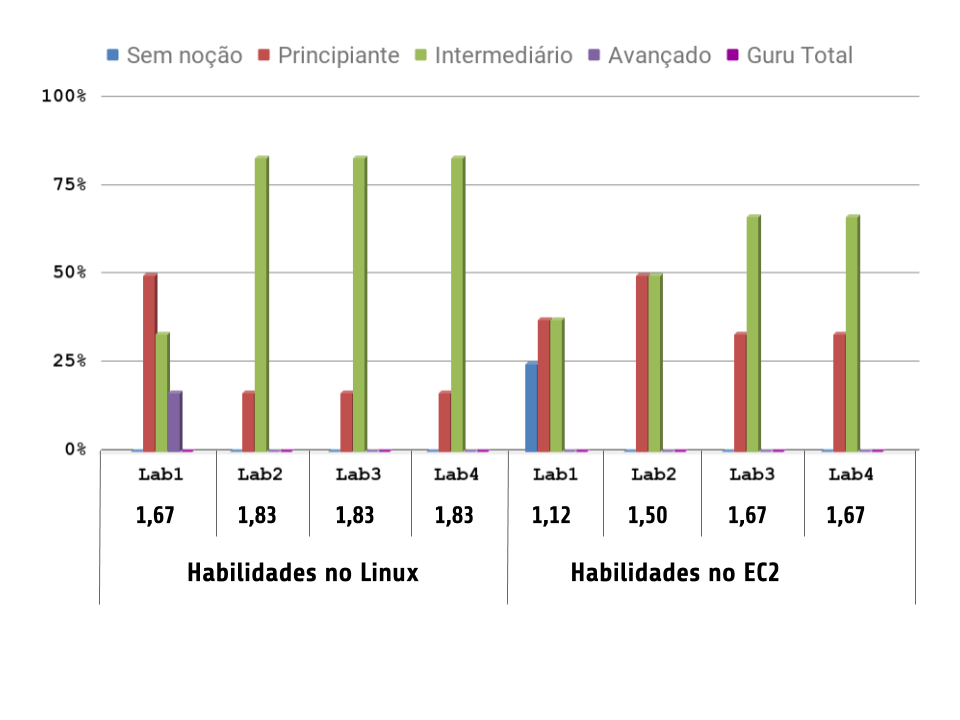
\includegraphics[width=16cm]{figuras/grafico-q1-q2.png}
		}{
			\Fonte{Próprio Autor.}
	}		
\end{figure}

Para obter o nível médio de habilidades, as cinco opções de respostas foram convertidas em valores numéricos, onde o nível 0 significa “Sem noção”, o nível 1 significa “Iniciante”, o nível 2 significa “Intermediário”, o nível 3 significa
“Avançado” e o nível 4 significa “Guru total”. Não existem escalas de intervalo, já que as respostas são ordinais. Essa conversão foi realizada simplesmente para facilitar a comparação dos níveis de habilidades de uma perspectiva relativa, após cada prática de laboratório. 

É possível observar que os exercícios  dessas quatro práticas de laboratório ajudaram o aluno a melhorar suas habilidades de uso do Linux e do EC2. A maioria dos alunos classificaram suas habilidades no Linux como principiante na prática de laboratório 1. O nível médio de habilidades no Linux aumento significativamente da prática de laboratório 1 para a prática de laboratório 2 e se manteve constante até a prática 4.
Em relação ao nível médio de habilidades no EC2, houve um aumento ainda maior da prática de laboratório 1 para a prática de laboratório 2, continuou aumentando para um nível de 1,67 na prática de laboratório 3, até que se manteve constante na prática de laboratório 4. Foi possível perceber que a maioria dos alunos teve alguma experiência no Linux antes de realizar a prática de laboratório 1, e ainda que apesar de todos os alunos terem declarados que não haviam utilizado algum serviço da Amazon Web Services anteriormente, após a prática de laboratório 1 uma porcentagem significativa dos estudantes se classificaram como nível intermediário.


\subsection{Resultados da pesquisa de Q3 e Q4}

Na segunda categoria do questionário estão inclusas duas perguntas fechadas, como mostrado na Tabela \ref{Tab:questionario}. A pergunta Q3 declara que as tarefas em uma prática de laboratório são difíceis. Os estudantes deveriam escolher uma das cinco opções de resposta: discordo fortemente, discordo, nem concordo nem discordo, concordo e concordo fortemente. A pergunta Q4 pede aos alunos para relatar o número de horas que eles gastaram para concluir as tarefas em uma prática de laboratório.

Na Figura \ref{fig:grafico-q3}, cada coluna representa a porcentagem de estudantes que escolheram cada opção de resposta correspondente a cada prática de laboratório em resposta a pergunta Q3. A Figura \ref{fig:grafico-q3eq4} ilustra o nível médio de dificuldade classificado pelos alunos nas tarefas de cada prática de laboratório e o número médio de horas trabalhadas em cada prática de laboratório. O nível médio de dificuldade é calculado usando a fórmula \ref{eq:form-q3}.


\begin{equation}\label{eq:form-q3}
nível \ medio \ de \ dificuldade = \sum_{i=1}^{5} (i*porcentagem \ de \ alunos \ que \ escolheram \ o \ nivel \ i)
\end{equation}



\begin{figure}[htb!] 
   	    \captionsetup{width=15cm}%Da mesma largura que a figura
		\Caption{\label{fig:grafico-q3} Avaliação da afirmação de que as tarefas em uma prática de laboratório são difíceis.}
		\UFCfig{}{
			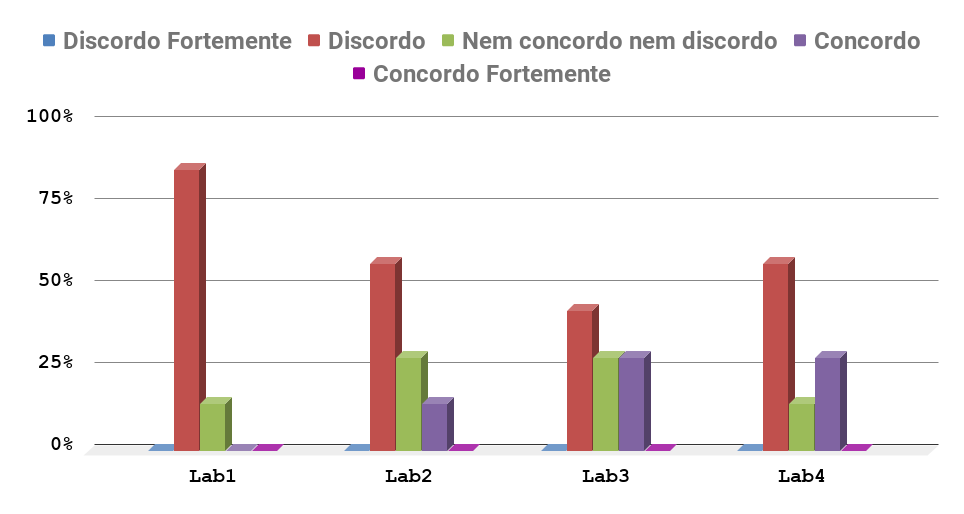
\includegraphics[width=16cm]{figuras/grafico-q3.png}
		}{
			\Fonte{Próprio Autor.}
	}		
\end{figure}

\begin{figure}[htb!] 
   	    \captionsetup{width=15cm}%Da mesma largura que a figura
		\Caption{\label{fig:grafico-q3eq4} Horas trabalhadas e nível médio de dificuldade das tarefas em cada prática de laboratório.}
		\UFCfig{}{
			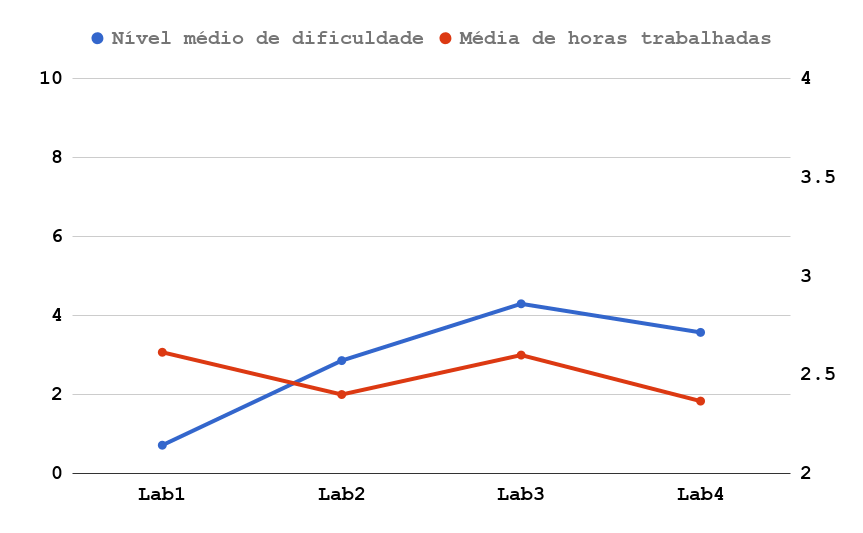
\includegraphics[width=16cm]{figuras/grafico-q3eq4.png}
		}{
			\Fonte{Próprio Autor.}
	}		
\end{figure}

Para obter o nível médio de dificuldade, as cinco opções de respostas foram convertidas em valores numéricos, onde o nível 1 significa “Discordo Fortemente”, o nível 2 significa “Discordo”, o nível 3 significa “Nem concordo nem discordo”, o nível 4 significa “Concordo” e o nível 5 significa “Concordo Fortemente”. Podemos ver na Figura \ref{fig:grafico-q3eq4} que no geral, o número médio de horas gastas pelos alunos em cada prática de laboratório concorda com o nível de dificuldade médio avaliado pelos alunos. O nível médio de dificuldade da prática 1 é menor do que o nível médio de dificuldade da pŕatica 2, contudo menos horas foram gastas no término da prática de laboratório 2. Considerando as curvas de aprendizado das habilidades do Linux e das habilidades do Amazon EC2 ilustradas na Figura \ref{fig:grafico-q1-q2}, essa  inconsistência é razoável, porque os alunos gastaram uma quantidade extra de tempo no aprendizado de Linux e do Amazon EC2. Os resultados também indicam que a prática de laboratório 3 é a mais desafiadora.

\subsection{Resultados da pesquisa de Q5, Q6, Q7 e Q8}

Na terceira categoria, quatro questões Q5, Q6, Q7 e Q8 (conforme a Tabela \ref{Tab:questionario}) foram fornecidas ao alunos para obter suas opiniões sobre o uso da instância EC2 F1. A Figura \ref{fig:grafico-q5-q6-q7-q8} ilustra os resultados obtidos dessas quatro perguntas. Cada coluna representa a porcentagem de estudantes que escolheram a opção de resposta para a pergunta correspondente em cada prática de laboratório, conforme listado na Tabela \ref{Tab:questionario}. O nível médio de concordância com o uso do Amazon EC2 é calculado usando a Fórmula \ref{eq:form-q4-q5-q6-q7-q8} e anotado acima do ID da pergunta, como mostrado na Figura \ref{fig:grafico-q5-q6-q7-q8}. 



\begin{equation}\label{eq:form-q4-q5-q6-q7-q8}
   nível \ medio \ de \ concordância = \frac{1}{4}\sum_{j=1}^{4} (\sum_{i=1}^{5} (i*\Delta)),
\end{equation}
onde $\Delta$ é porcentagem de alunos que escolheram o nível i no lab j.




\begin{figure}[htb!] 
   	    \captionsetup{width=15cm}%Da mesma largura que a figura
		\Caption{\label{fig:grafico-q5-q6-q7-q8} Ranking de concordância com o uso do Amazon EC2.}
		\UFCfig{}{
			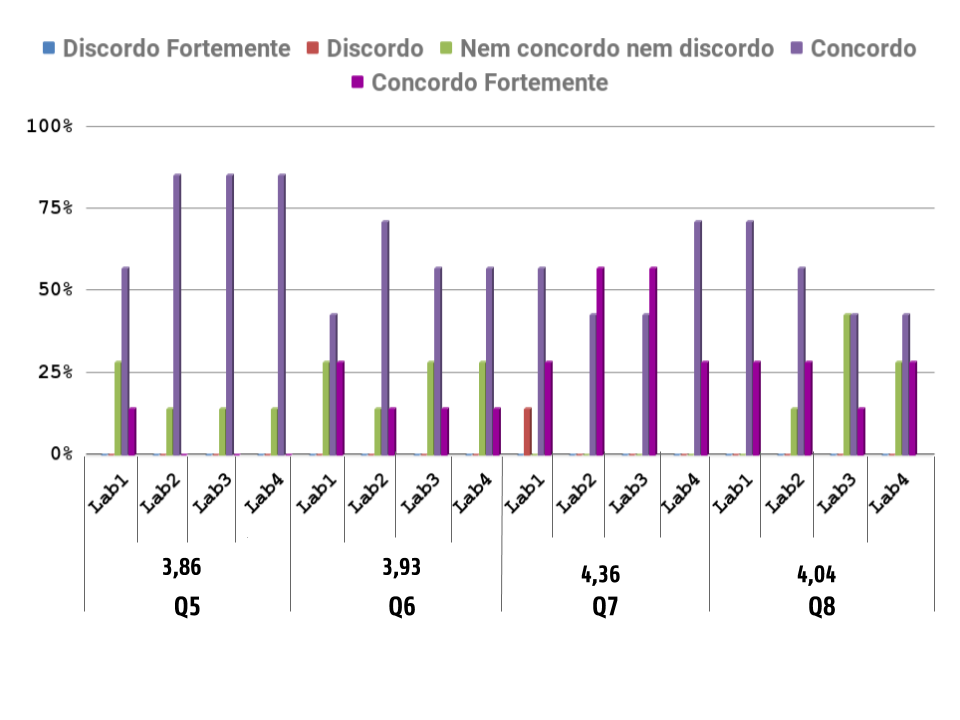
\includegraphics[width=16cm]{figuras/grafico-q5-q6-q7-q8.png}
		}{
			\Fonte{Próprio Autor.}
	}		
\end{figure}

Para obter o nível médio de concordância, as cinco opções de respostas foram convertidas em valores númericos, de maneira idêntica a que foi feita na Fórmula \ref{eq:form-q3}. É possível perceber que a porcentagem de alunos que escolheram a opção "Concordo" permance a mais alta em cada prática de laboratório, exceto para a pergunta Q8 na prática de laboratório 3. Não houveram alunos que escolheram a opção "Discordo fortemente" ou a opção "Discordo", portanto, é possível concluir que a maioria dos alunos  gostaria de usar o Amazon EC2 F1 em exercícios de laboratório de SEDR semelhantes no futuro (Q5), considera a experiência de uso do Amazon EC2 F1  útil para o desenvolvimento de suas carreira (Q6) e usaria o Amazon EC2 F1 em pesquisas/trabalhos no futuro (Q8).

Coom relação à afirmação de que é importante para o aprendizado da disciplina o uso remoto de uma FPGA \textit{high end} (Q7), na primeira prática de laboratório 14,3\% dos alunos discordam com a afirmação, em contra partida, a porcentagem de estudantes que concordam  e concordam fortemente com a afirmação é de 57,1\% e 28,6\%, respectivamente. Além disso, a porcentagem dos alunos que concordam fortemente continua a crescer e não há mais alunos que dicordam nas práticas de laboratório seguintes. Com isso, é possível concluir que a maioria dos estudantes concorda com a importância do uso remoto de uma FPGA  \textit{high end}. 

Quanto à declaração sobre o uso do Amazon EC2 F1 em pesquisas/trabalhos no futuro, 14,3\% dos alunos responderam que nem concordam nem discordam, na prática de laboratório 2, essa porcentagem aumentou para 42,9\% na prática de laboratório 3 e diminuiu para 28,6\% na prática de laboratório 4. Com isso, pode-se dizer que alguns alunos podem ter receio sobre o uso das instâncias EC2 F1 em outras atividades mesmo depois de terem acumulado experiência nas práticas de laboratório. Portanto, acredita-se que uso do Amazon EC2 F1 é benéfico dependendo da natureza da pesquisa ou do trabalho que será realizado.

\subsection{Resultados da pesquisa de  perguntas abertas}

No questionário estão inclusas duas perguntas abertas Q9 e Q10, conforme mostrado na Tabela \ref{Tab:questionario}, a fim de permitir que os alunos comentem abertamente sobre o uso do Amazon EC2 F1 nas práticas de laboratório. A pergunta Q9 trata-se da parte mais difícil para concluir as tarefas em cada prática usando a Amazon EC2. Uma opinião comum indicada pelos comentários dos alunos nas quatro práticas de laboratório é que a falta de experiência com o uso dos comandos necessários para se utilizar o serviço EC2 F1 torna a prática complicada no primeiro momento, mas o uso contínuo dos comandos torna mais fácil a execução das tarefas das práticas de laboratório. Este resultado é consistente com o progresso do nível médio de habilidades no EC2 ilustrado na Figura \ref{fig:grafico-q1-q2}. Três comentários representativos fornecidos pelos alunos à pergunta Q9 são citados diretamente abaixo:


\textit{"A principio, por falta de experiência, o passo a passo é um pouco complicado, mas com o uso fica melhor."}

\textit{"A parte de pedir a instância F1. Mas só porque os comandos são longos e fáceis de confundir. No mais, é tudo muito tranquilo e bem explicado."}

\textit{"Os primeiros contatos com a interface gráfica e a utilização da máquina virtual, o que não foi problemático."}

Houveram alguns comentários negativos em resposta à pergunta Q9, que diz respeito ao tempo disponível para a realização das práticas e a quantidade de tarefas das mesmas. Isso é mostrados nos comentários citados abaixo:

\textit{"Muita atividade e pouco tempo."}

\textit{"Muitas etapas."}

\textit{"Tempo curto."}

É importante destacar alguns comentários específicos da prática de laboratório 4, que mostram que parte da dificuldade de completar as tarefas dessa prática deve-se à falta de recursos computacionais do laboratório para executar a máquina virtual que contém o ambiente de desenvolvimento fornecido pela Amazon Web Services. Alguns desses comentários são citados abaixo:

\textit{"A máquina virtual usada era lenta e alterou alguns valores de endereçamento."}

\textit{"Execução do Vivado em máquinas lentas torna o laboratório desnecessariamente complicado."}

\textit{"A falta de recurso computacional adequado compromete muito a prática."}


A última pergunta Q10 simplesmente pede que os alunos forneçam quaisquer comentários e sugestões sobre cada prática de laboratório em particular e do Amazon EC2 F1. Houveram poucas respostas para essa pergunta, no geral, os alunos ficaram empolgados para exemplos mais complexos na prática de laboratório 1, sugeriram melhoras na descrição da prática e acreditam que com os recursos computacionais adequados tornam as práticas de laboratório 3 e 4 ainda mais interessantes. Três comentários representativos fornecidos pelos alunos na pergunta Q10 são diretamente citados abaixo: 

\textit{"Achei muito interessante. Com a eventual melhora dos laboratório pra fazerem exemplos mais complexos, vai ficar muito bom."}

\textit{"As prática em texto, como todas as práticas de texto aplicadas em qualquer disciplina, são um pouco superficiais, não dando um entendimento completo do que se está fazendo. Uma explanação passo a passo antes da realização da prática seria interessante."}

\textit{"A prática fica legal quando feita com os recursos certos."}

\section{Modificações nas práticas}\label{sec:modificacoes-nas-praticas}

Após a a aplicação de cada prática, percebeu-se a necessidade de algumas alterações nas mesmas. No entanto, foram alterações mínimas, que dizem respeito apenas a modificação do formato dos comandos informados nas práticas, de forma que se tornasse mais intuitivo na hora de usá-los.


	\chapter{Considerações Finais}
\label{chap:conclusoes-e-trabalhos-futuros}
Este trabalho apresentou a experiência do serviço Amazon EC2 F1 como uma ferramenta para o ensino de FPGAs através de quatro práticas de laboratório. Além disso,  foram apresentados os recursos e vantagens relacionados a esse serviço, foram fornecidos detalhes sobre o procedimento para usar as instâncias de desenvolvimento e a F1, foi apresentado o conteúdo das quatro práticas de laboratório, além de terem sido discutidos os resultados da pesquisa sobre o uso do Amazon EC2 F1, facilitando a experiência de educadores que desejam utilizar esse serviço para o ensino de FPGAs.

Os resultados indicam um aumento significativo do nível médio de habilidades no Amazon EC2, e mostram que, de uma maneira geral, os alunos se mostraram empolgados em aprender sobre o Amazon EC2 na disciplina, além de considerarem uma experiência útil para o desenvolvimento de suas carreiras. Porém, identificou-se um certo receio por parte dos alunos no uso das instâncias EC2 F1 em outras pesquisas ou trabalhos, o que leva a acreditar que os benefícios do uso do Amazon EC2 F1 variam de acordo com a natureza da pesquisa ou trabalho a ser realizado.

Observamos também que a maioria dos alunos não são versados no uso do sistema operacional linux, o que dificulta bastante o aprendizado das instâncias EC2 F1. Ainda que o objetivo da disciplina de SEDR esteja longe de querer ensinar o uso do Linux, foi possível observar uma melhoria expressiva do conhecimento dos alunos nesse sentido.

Com relação ao conteúdo abordado nas práticas, observou-se que uma parte da dificuldade do entendimento das práticas se deve a falta de conhecimento prévio de conceitos relacionados ao desenvolvimento de aplicações para FPGAs. Por exemplo, antes do início das práticas, a disciplina incluiu apenas uma explanação básica sobre barramentos AXI. Tendo em vista que a arquitetura imposta pela Xilinx para uso na EC2 F1 é essencialmente baseada nesse tipo de interface, recomenda-se a inclusão de um maior número de horas teóricas previamente à execução das práticas, detalhando os diversos tipos de barramentos AXI, a saber, AXI Stream, AXI Lite e AXI Full. Mais ainda, recomenda-se a inclusão de práticas com interface AXI utilizando a placa Basys 3 usada na disciplina. Da mesma forma, recomenda-se que as práticas anteriores às práticas da EC2 F1, sejam já executadas em ambiente linux, mas não em ambiente windows, e que incluam o uso de interface tcl em modo batch do Vivado, o que facilita bastante o aprendizado das instâncias EC2 F1.



\section{Limitações e Trabalhos Futuros}\label{sec:limitacoes-e-trabalhos-futuros}
Para ter acesso ao serviço EC2 F1 e receber o \textit{voucher} de USD\$ 100,00 , o aluno precisa fornecer um cartão de crédito, o que dificulta bastante a adesão dos alunos a este modelo. Neste sentido, recomenda-se a elaboração e subsmissão de projeto educacional a fim de receber créditos para que os alunos possam fazer as práticas sem nenhum custo, e sem precisar informar um número de cartão de crédito.

Além disso, nas práticas 3 e 4, A simulação e verificação do sistema \textit{shell/custom logic} foi executado localmente nas máquinas do laboratório de hardware. Observou-se uma lentidão exagerada, o que causou travamentos e mesmo desestímulo nos alunos. Neste sentido, recomenda-se o uso de máquinas com recursos computacionais superiores, com pelo menos de 8GB de memória RAM. 

Observou-se ainda que a internet da UFC não forneceu uma conexão adequada para permitir o uso com fluidez da interface gráfica do vivado, sendo executado remotamente nas instâncias da Amazon.

Como trabalhos futuros, é sugerido a elaboração de práticas baseadas em ferramentas de desenvolvimento em alto nível, tal como SDAccell e Vivado HLS, o que permite o desenvolvimento rápido de sistemas mais complexos, permitindo ao aluno compreender melhor o verdadeiro potencial computacional das EC2 F1. Além de práticas que permitam o debug remoto do hardware usando a virtual JTAG.








	
	%Elementos pós-textuais	
	\bibliography{3-pos-textuais/referencias}
%	\imprimirglossario	
	\imprimirapendices
		% Adicione aqui os apendices do seu trabalho
		\apendice{Roteiro das práticas de laboratório}
\label{ap:A}

Os roteiros das práticas também estão disponíveis no GitHub, no link: \url{https://github.com/vanros/Praticas-SEDR-AWS}.


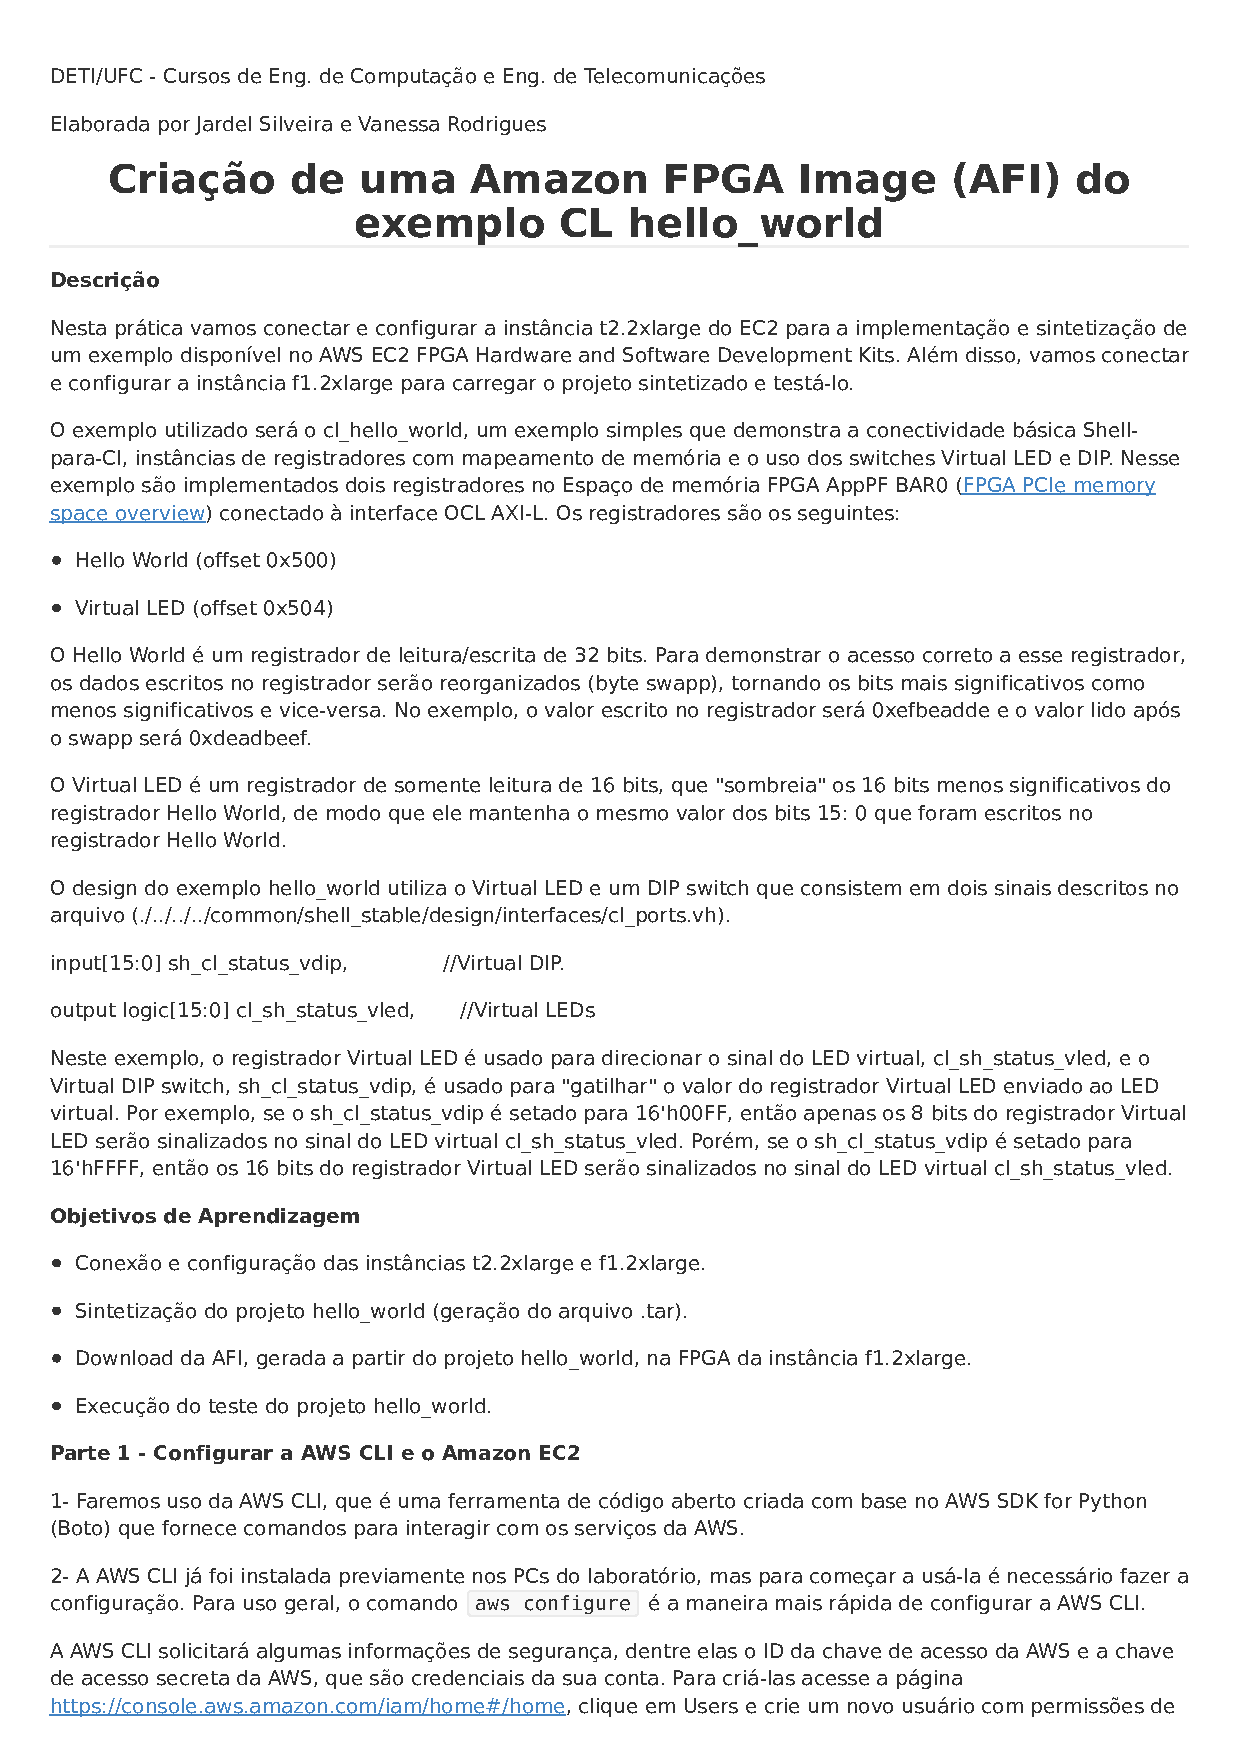
\includepdf[pages={-}]{3-pos-textuais/apendices/Pratica1.pdf}

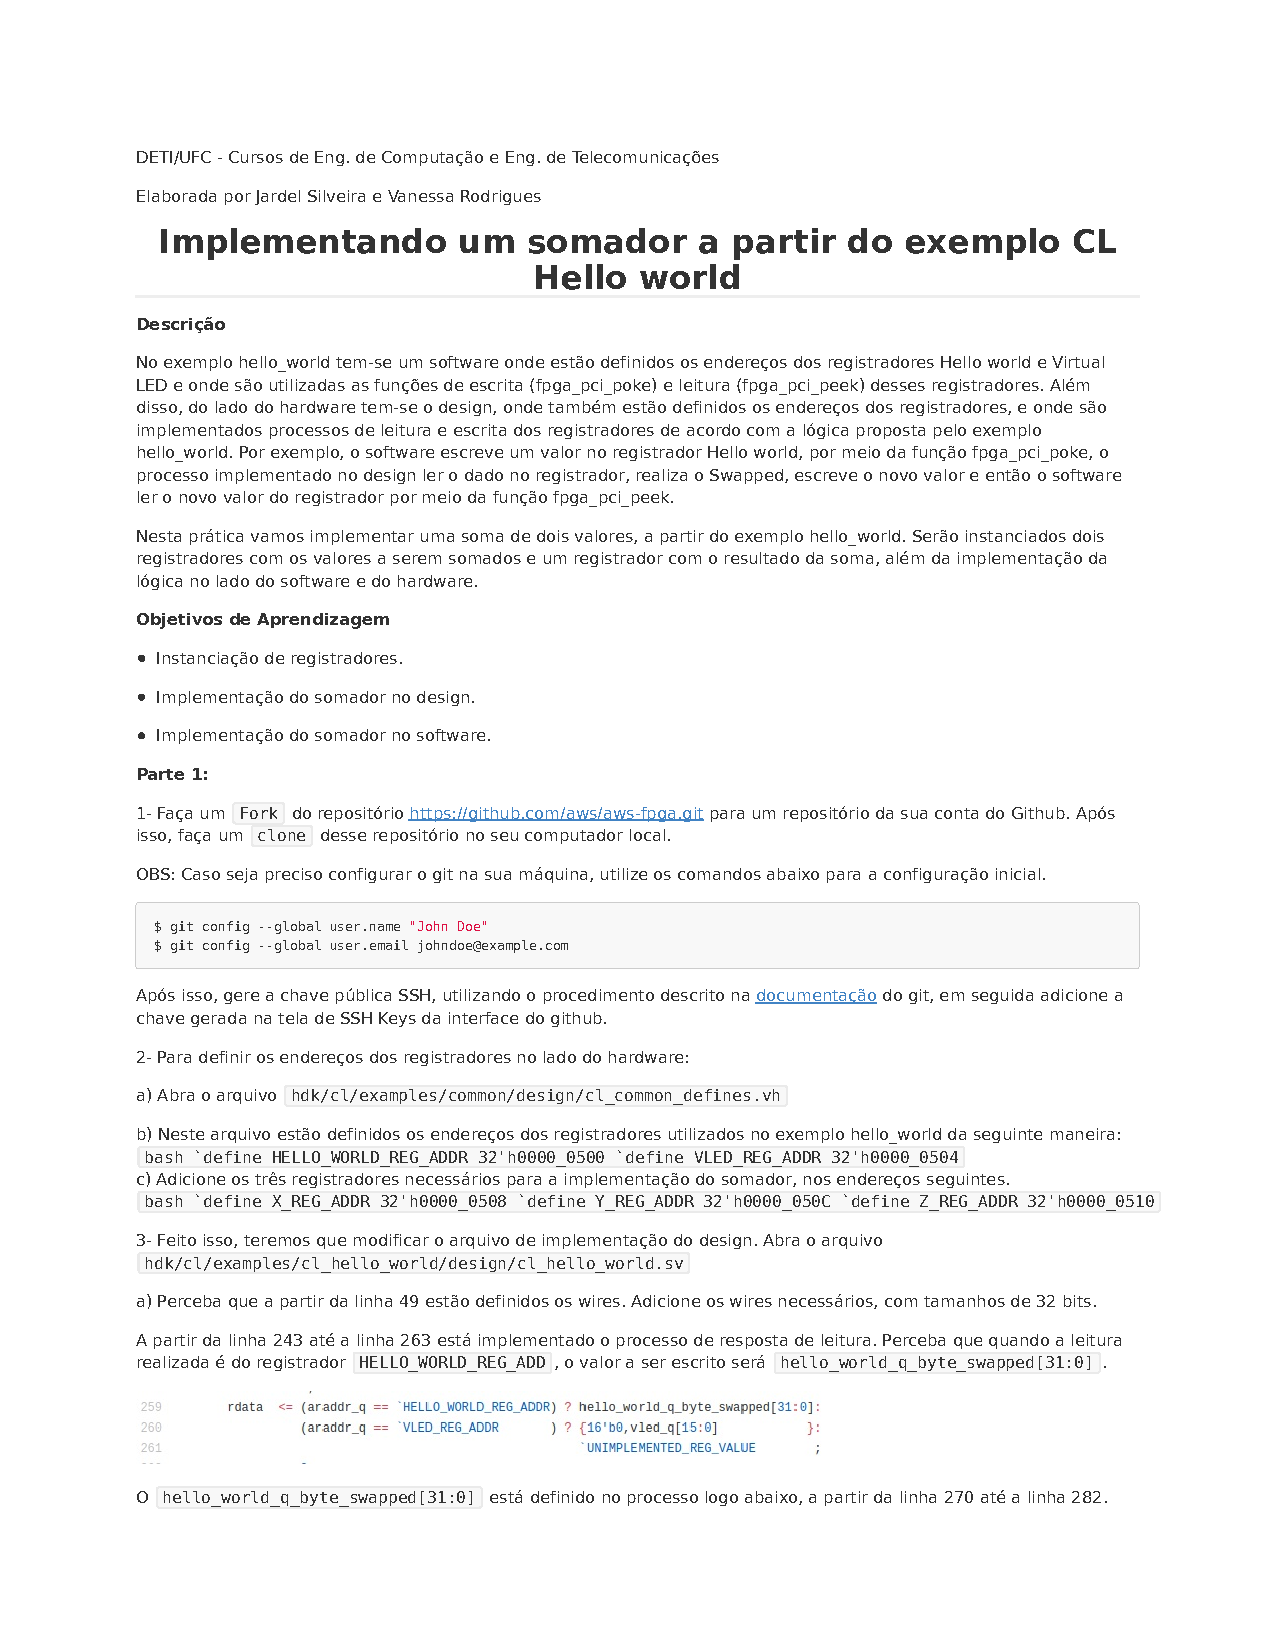
\includepdf[pages={-}]{3-pos-textuais/apendices/Pratica2.pdf}

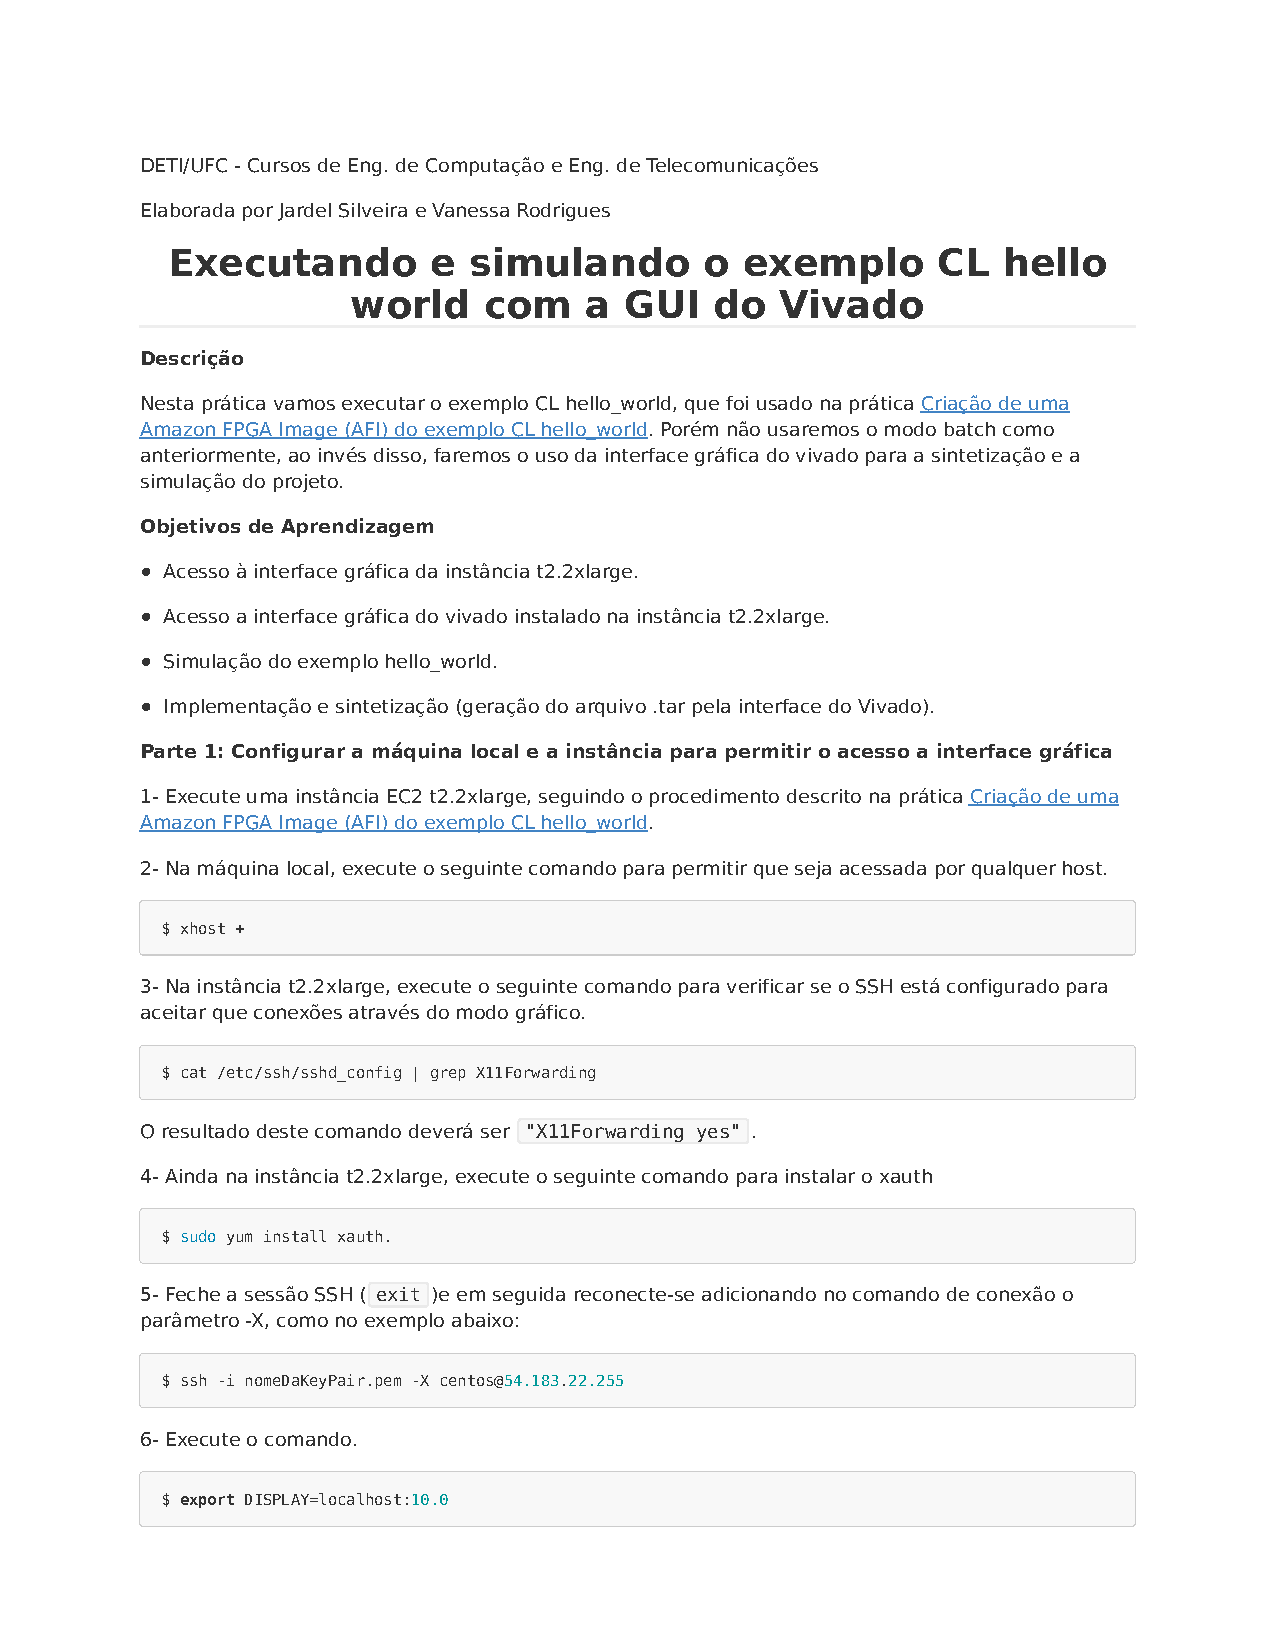
\includepdf[pages={-}]{3-pos-textuais/apendices/Pratica3.pdf}

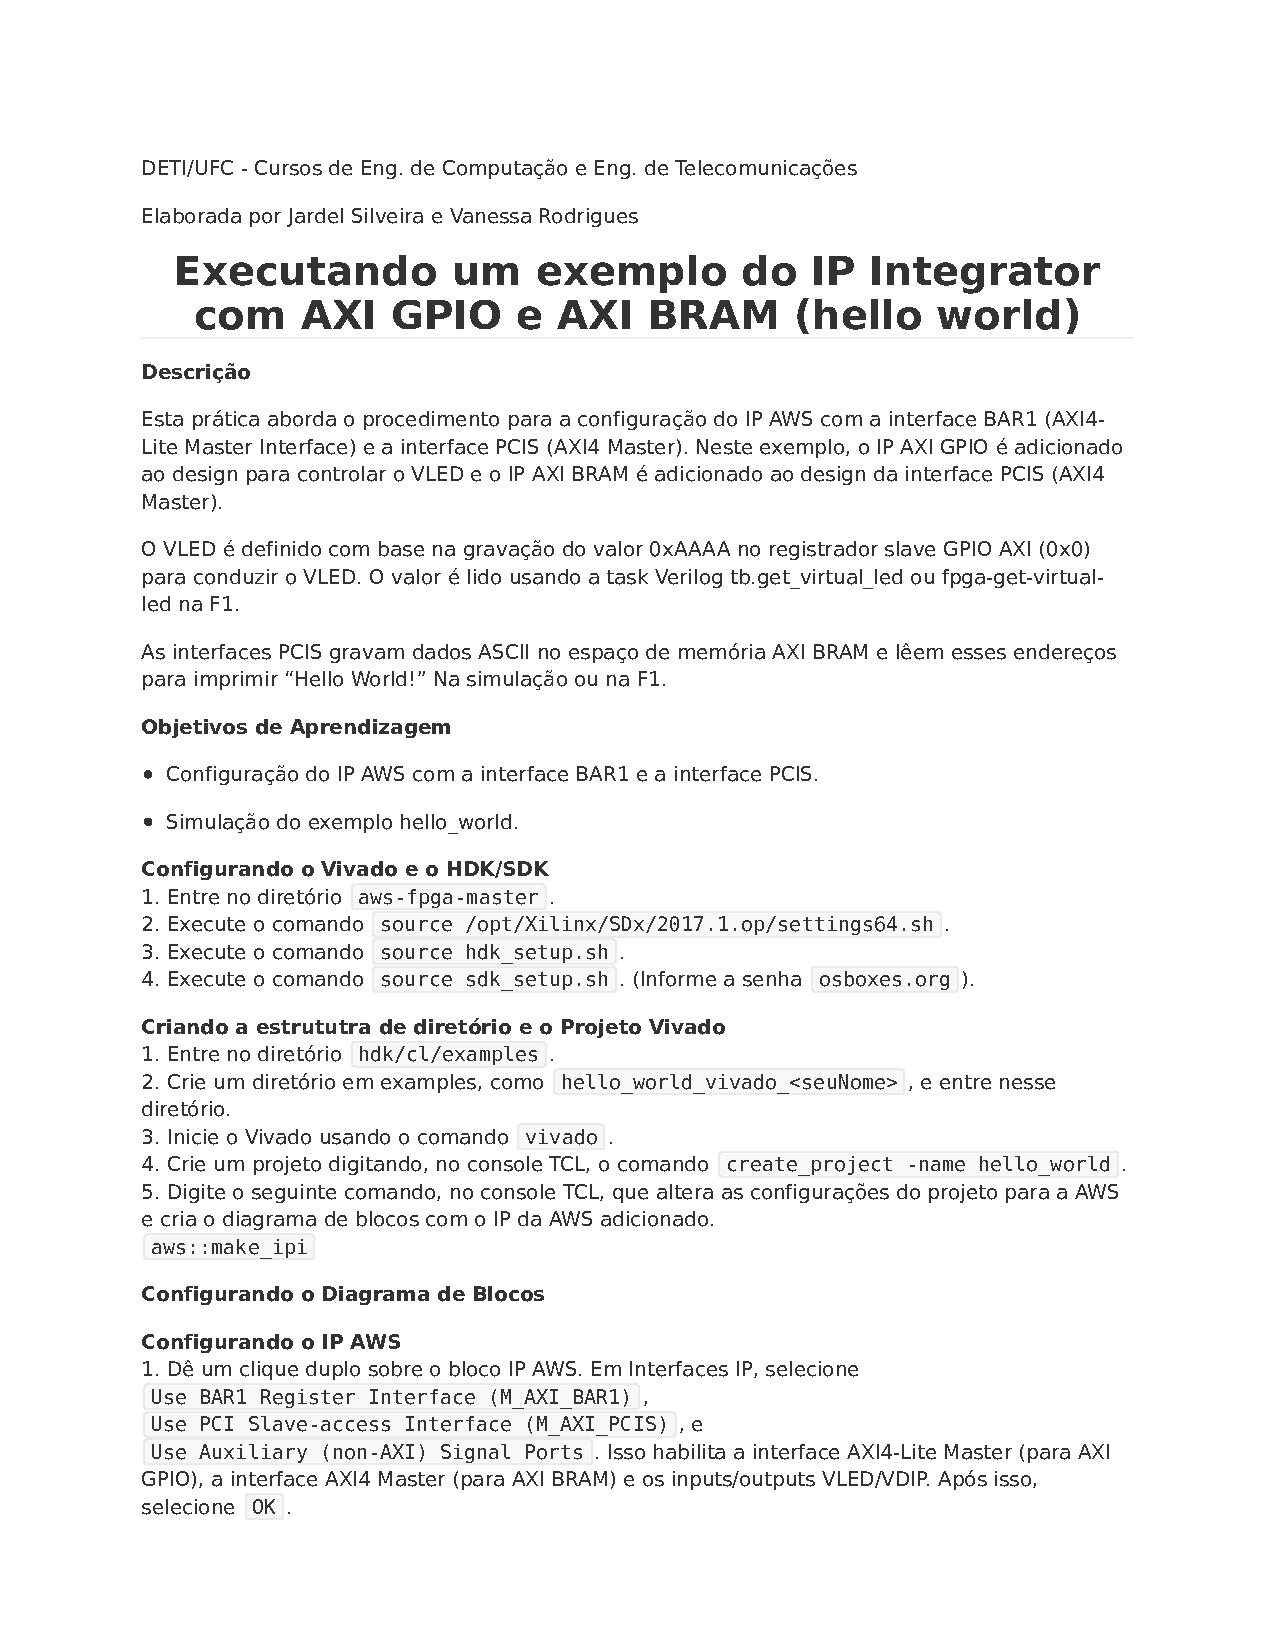
\includepdf[pages={-}]{3-pos-textuais/apendices/Pratica4.pdf}
	%	\apendice{Questionário utilizado para...}
\label{ap:B}

\begin{questao}
	\item Esta é a primeira questão com alguns itens:
		\begin{enumerate}
			\item Este é o primeiro item
			\item Segundo item
		\end{enumerate}
	\item Esta é a segunda questão:
		\begin{enumerate}
			\item Este é o primeiro item
			\item Segundo item
		\end{enumerate}
	\item Lorem ipsum dolor sit amet, consectetur adipiscing elit. Nunc dictum sed tortor nec viverra. consectetur adipiscing elit. Nunc dictum sed tortor nec viverra.
		\begin{enumerate}
			\item consectetur
			\item adipiscing
			\item Nunc
			\item dictum
		\end{enumerate}
\end{questao}

	%	\apendice{Códigos-fontes utilizados para...}
\label{ap:C}

\lstinputlisting[language=C++,caption={Hello World em C++}]{figuras/main.cpp}


\begin{lstlisting}[language=Java,caption={Hello World em Java}]
public class HelloWorld {
	public static void main(String[] args) {
		System.out.println("Hello World!");
	}
}
\end{lstlisting}


	%	\apendice{\textit{IEEE CEFC 2016}}
\label{ap:D}

\textit{Digest} submetido ao \textit{The 17th Biennial Conference on Eletromagnetic Field Computation, Miami FL - NOV 13-16, 2016, USA}.

%Código fonte para inserir um arquivo em PDF
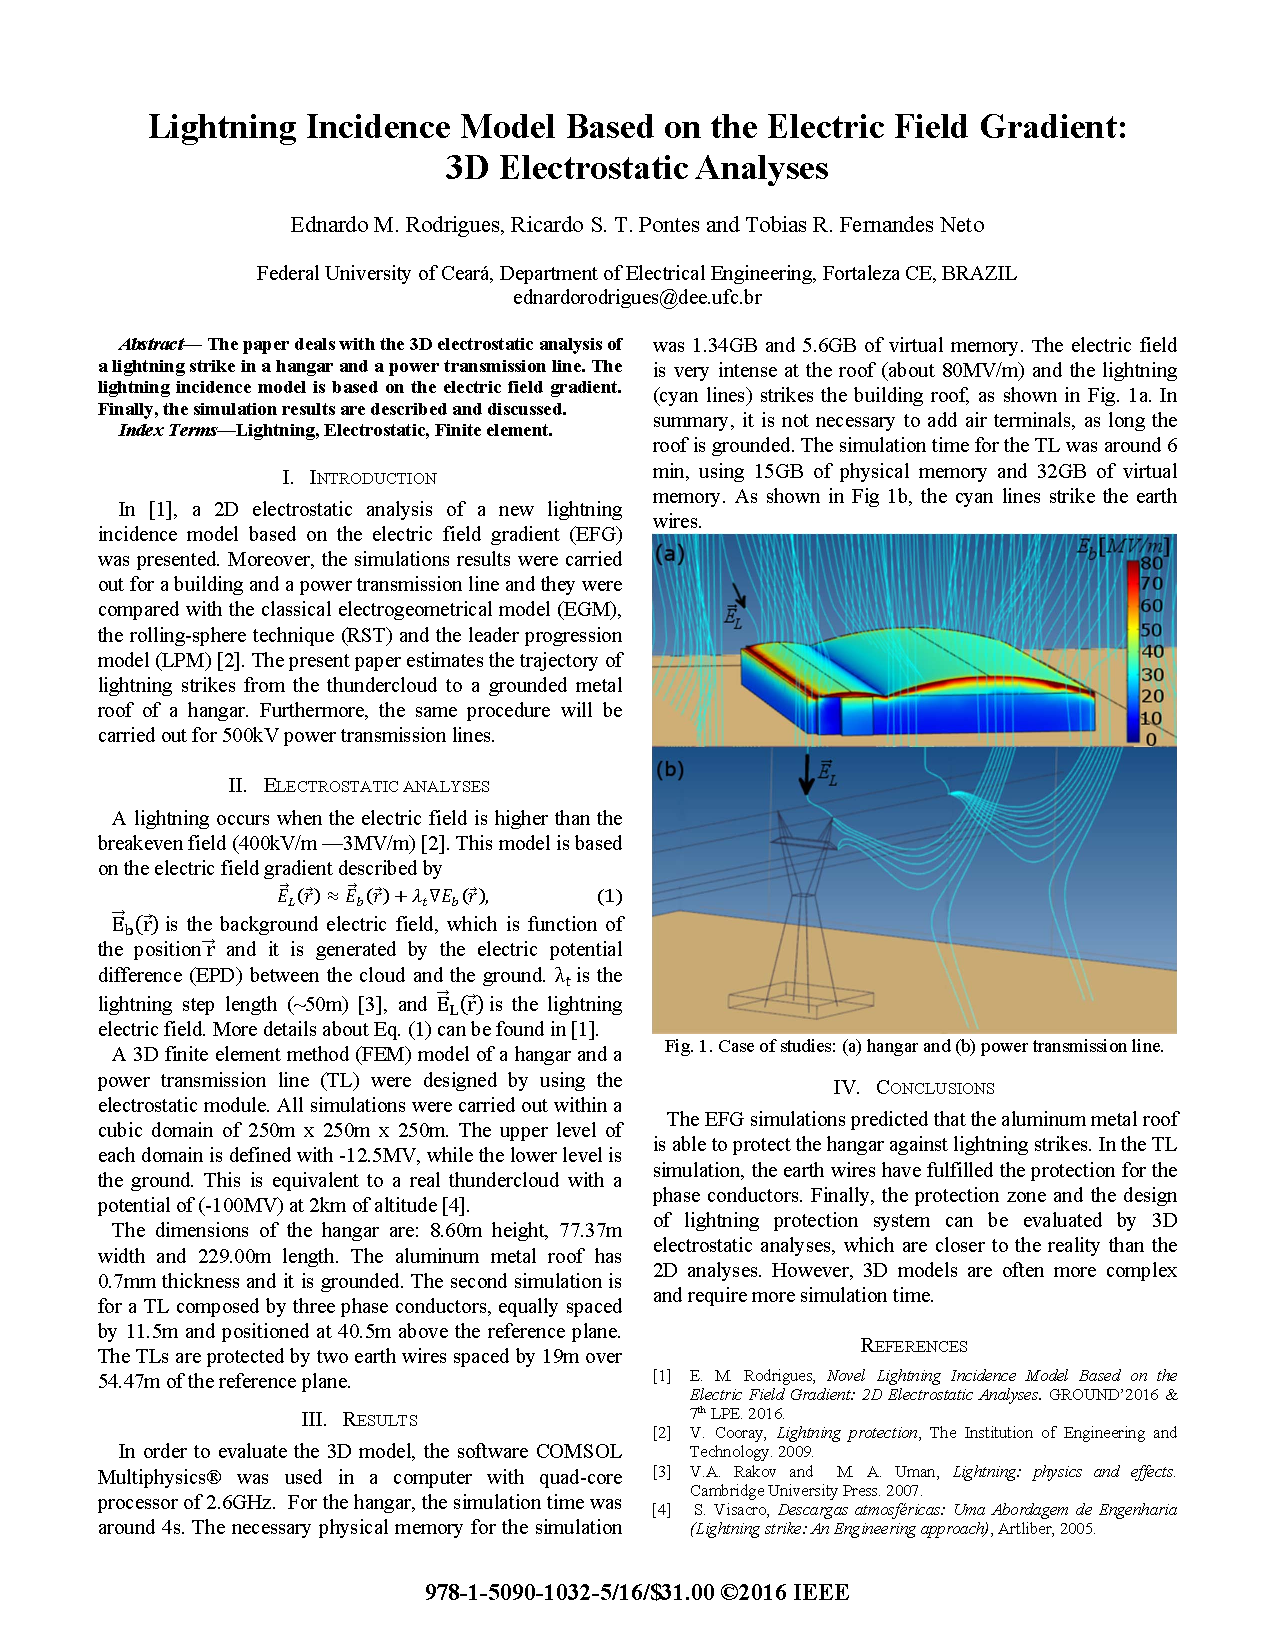
\includepdf[pages={-}]{3-pos-textuais/apendices/PID4416093.pdf}
	\imprimiranexos
		% Adicione aqui os anexos do seu trabalho
		\anexo{Ementa da Disciplina de Sistemas Eletrônicos Digitais Reconfiguráveis}
\label{an:ex_anexo_a}

Ementa da disciplina de sistemas eletrônicos digitais reconfiguráveis.

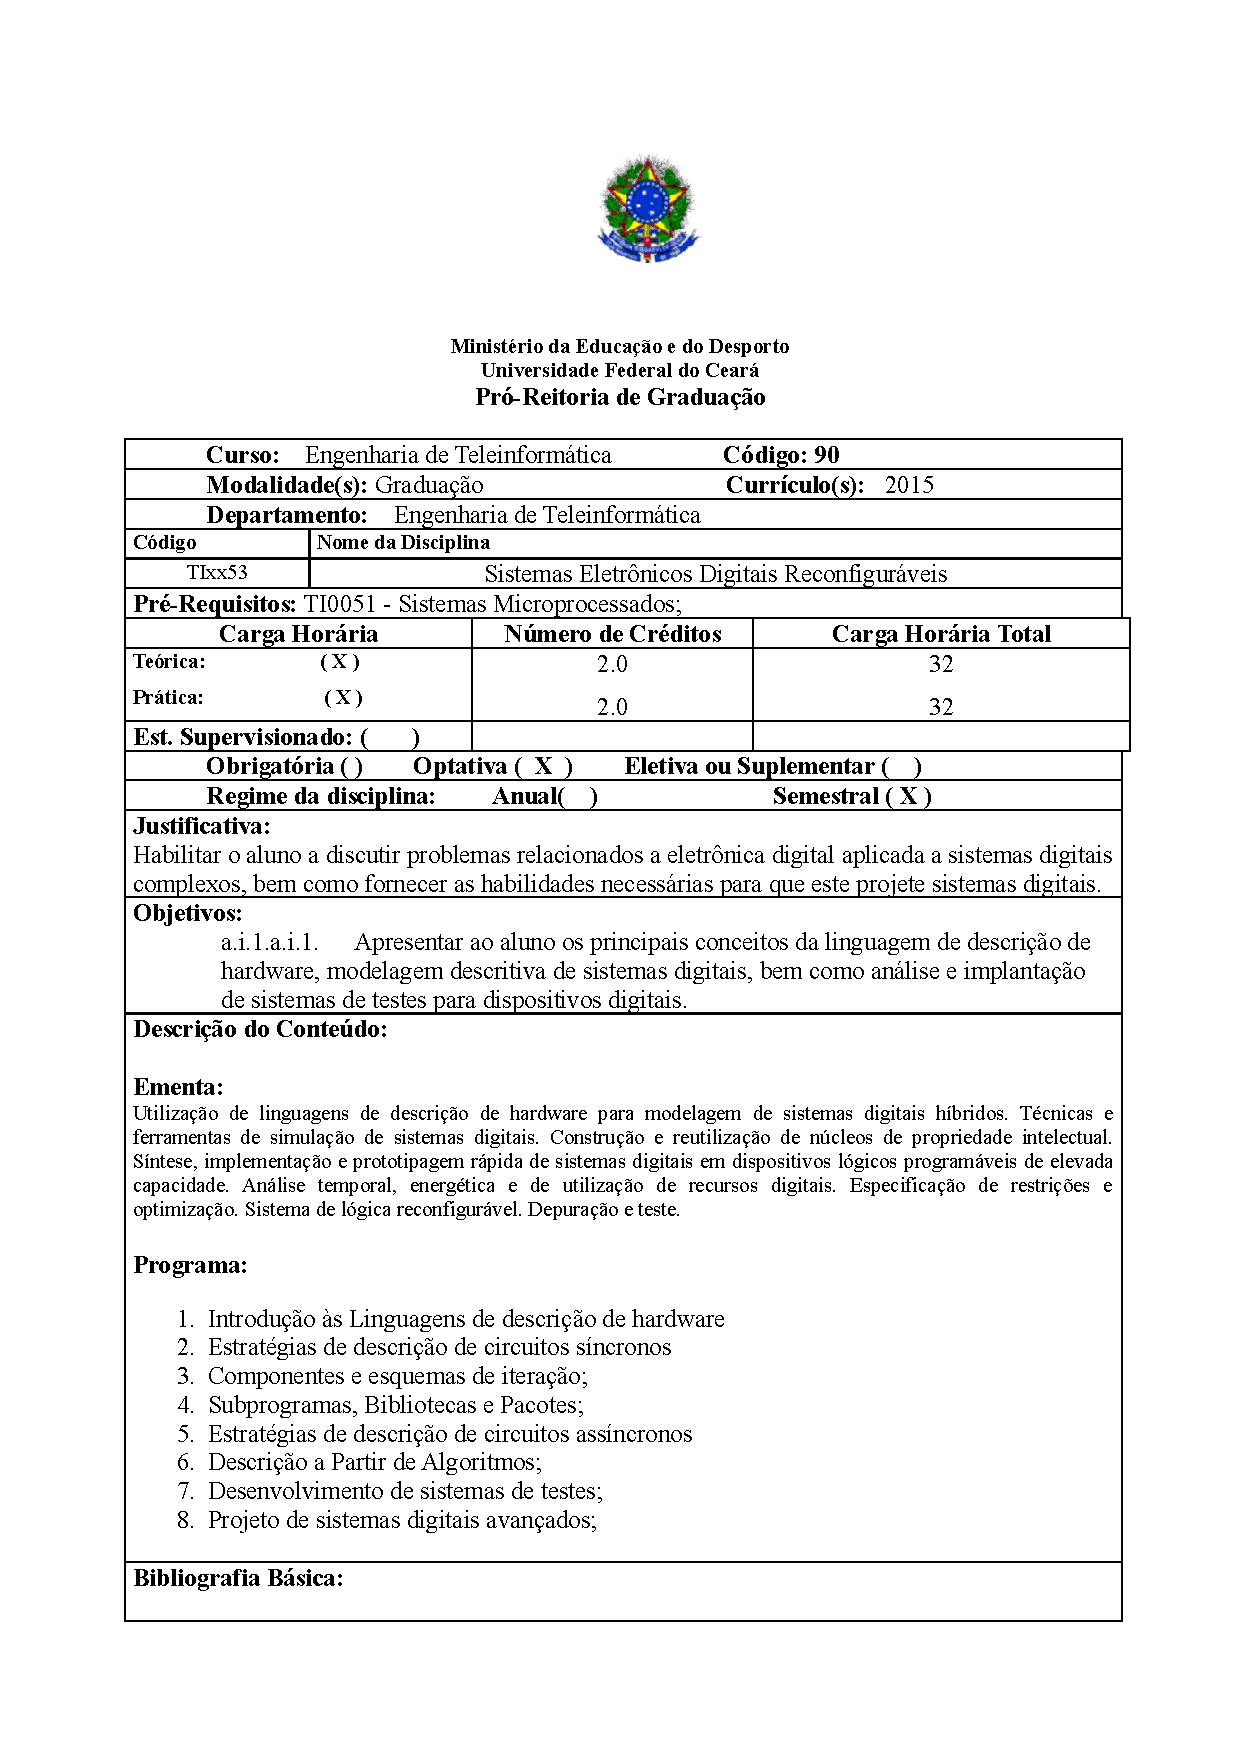
\includepdf[pages={-}]{3-pos-textuais/anexos/sistemas-eletronicos-digitais-reconfiguraveis.pdf}


	%	\anexo{Exemplo de um anexo em PDF}
\label{an:ex_anexo_b}

O autor pode anexar um \gls{PDF}, traduzido como formato portátil de documento. Veja o código fonte utilizado para anexar o arquivo ``Sikasil.pdf'' que foi colocado dentro da pasta ``anexos'' que por sua vez está dentro da pasta ``elementos-pos-textuais''. Tenha muita atenção na hora de especificar o local do arquivo. Recomenda-se não utilizar caracteres especiais para nomear pastas e, principalmente, arquivos. 

Pode-se fazer uma descrição sucinta do arquivo anexado.

%Comando para incluir um arquivo em PDF:
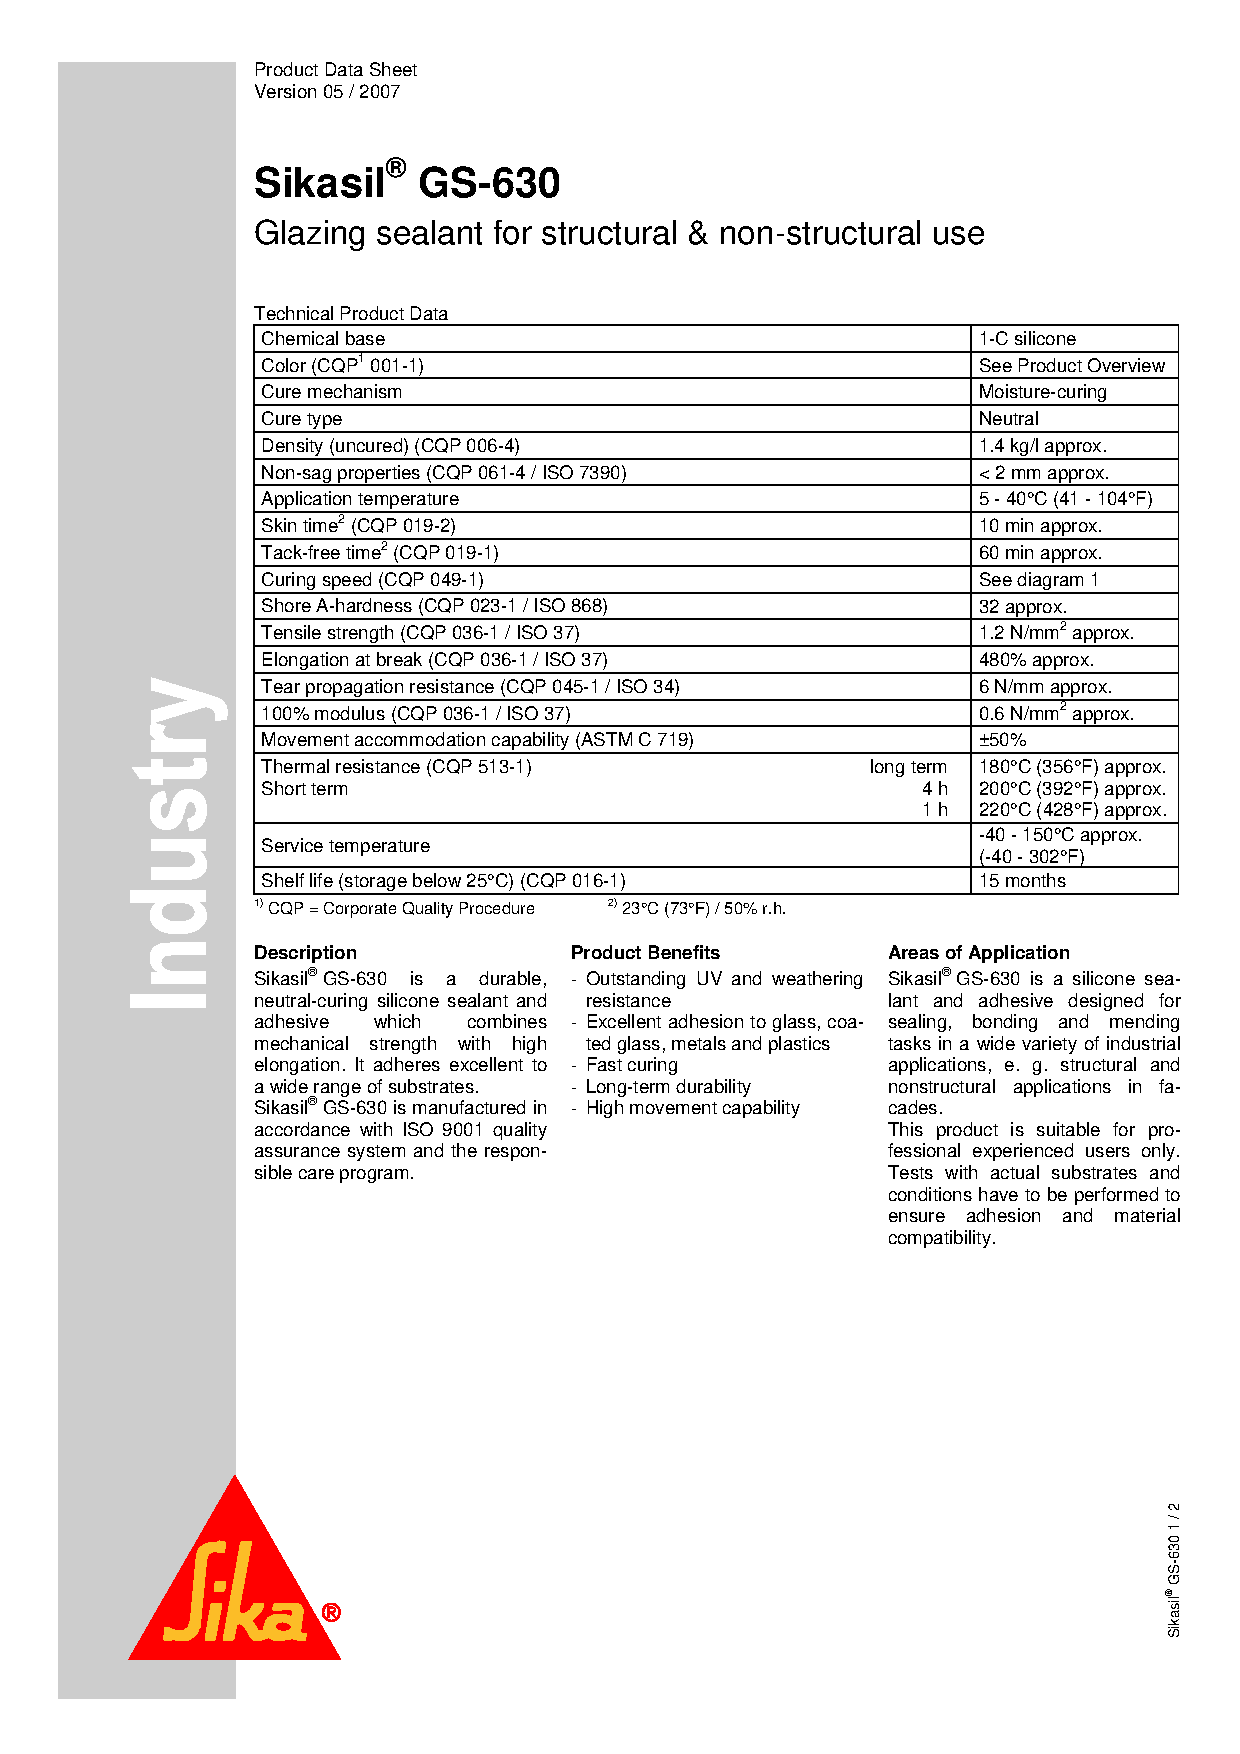
\includepdf[pages={-}]{3-pos-textuais/anexos/Sikasil.pdf}

		
	\imprimirindice

\end{document}